\documentclass[aspectratio=169]{beamer}
\usetheme{Copenhagen}
\usecolortheme{whale}
\usefonttheme[onlymath]{serif}
\addtobeamertemplate{footnote}{\hskip -2em}{}

\usepackage{setspace}
\usepackage{xcolor}
\usepackage{graphicx}
\usepackage{multimedia}
\usepackage{fontawesome5}
\usepackage[most]{tcolorbox}
\usepackage{empheq}
\usepackage{fancybox}
\usepackage{annotate-equations}
\usepackage{soul}
\usepackage{tikz}
\usetikzlibrary{positioning, calc, shapes.geometric, shapes.multipart, 
	shapes, arrows.meta, arrows, 
	decorations.markings, external, trees}
\tikzstyle{Arrow} = [
thick, 
decoration={
	markings,
	mark=at position 1 with {
		\arrow[thick]{latex}
	}
}, 
shorten >= 3pt, preaction = {decorate}
]

\definecolor{teel}{HTML}{00AEB3}
\definecolor{redorange}{HTML}{F26035}
\definecolor{darkred}{HTML}{8B0000}
\definecolor{darkblue}{HTML}{00008B}
\definecolor{darkgreen}{HTML}{06402B}
\definecolor{CarolinaBlue}{HTML}{4B9CD3}

\usecolortheme[named=CarolinaBlue]{structure}

\title[Math Models]{Assumptions, Information, and What We Learn from Different Models}
\author[Zivich]{Paul Zivich \\ Assistant Professor \\ Department of Epidemiology \\ University of North Carolina at Chapel Hill}

\setbeamercovered{transparent}
\setbeamertemplate{navigation symbols}{}  % gets rid of the dumb navigation symbols
\setbeamertemplate{page number in head/foot}{\insertframenumber}  % adds slide #
\setbeamertemplate{headline}{}

\newcommand\blfootnote[1]{%
	\begingroup
	\renewcommand\thefootnote{}\footnote[frame]{#1}%
	\addtocounter{footnote}{-1}%
	\endgroup
}

\AtBeginSection[]{
	\begin{frame}
		\vfill
		\centering
		\begin{beamercolorbox}[sep=8pt,center,shadow=true,rounded=true]{title}
			\usebeamerfont{title}\insertsectionhead\par%
		\end{beamercolorbox}
		\vfill
	\end{frame}
}

\begin{document}
	
\begin{frame}[plain]
	\maketitle
\end{frame}

\begin{frame}{About Me\footnote[frame]{Footnotes are for asides or references}}
	\begin{columns}
		\begin{column}{0.35\textwidth}
			\begin{center}
				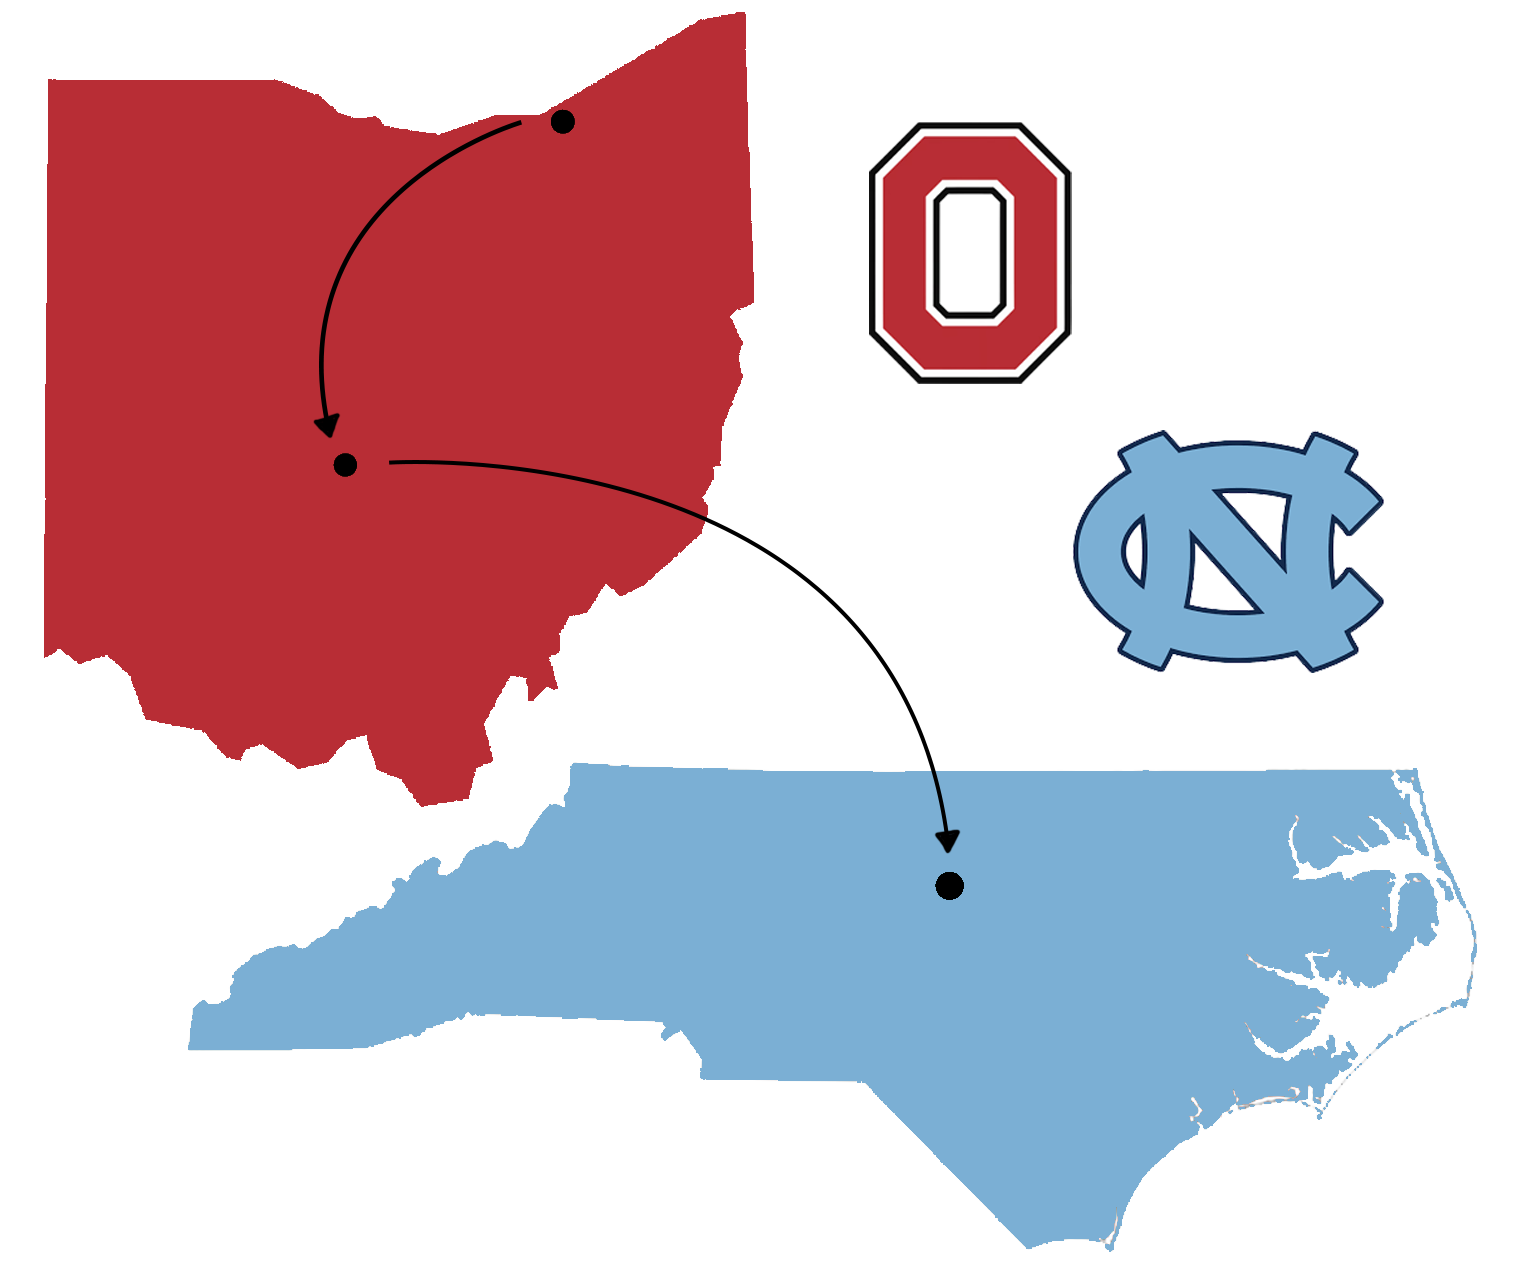
\includegraphics[width=0.95\linewidth]{images/places_ive_lived.png}
			\end{center}
		\end{column}
		\begin{column}{0.65\textwidth}
			\textbf{Research}
			~\\
			\textit{Methods}: causal inference, alternative randomized trial designs, estimating equations, data fusion 
			~\\~\\
			\textit{Applied}: infectious diseases (HIV, respiratory), pharmacoepidemiology, social epidemiology
		\end{column}
	\end{columns}
	~\\~\\
	\begin{center}
		\small
		\faEnvelope \quad pzivich@unc.edu \qquad \quad 
		\faGithub \quad pzivich \qquad \quad
		\faHashtag \quad pausalz@bsky.social
	\end{center}
	\begin{center}
		Zivich PN \textit{arXiv:2511.01960}
	\end{center}
\end{frame}

\begin{frame}{A Familiar Scenario(?)}
	Two research groups attempt to answer the same (a similar) question
	\begin{itemize}
		\item Use different study designs or methods
		\item End up with substantively different answers
	\end{itemize}
	~\\
	Differences can arise even when research groups do everything `right'
	\begin{itemize}
		\item Want to explain why we get different answers
	\end{itemize}
	~\\
	\textbf{Example}: trial versus observational for hormone replacement therapy
	\begin{itemize}
		\item Trial found greater coronary heart disease, while observational found lower
		\item Differences due to underlying populations (e.g., time since menopause)\footnote[frame]{Hern\'an et al. \textit{Epidemiology} 2008; 19(6):766-779}
	\end{itemize}
\end{frame}

\begin{frame}{Two Traditions of Modeling}
	Statistical (phenomenological) modeling
	\begin{itemize}
		\item Use observations to estimate parameters of a model
		\item \textbf{Examples}: randomized trials, regression, inverse probability weighting
	\end{itemize}
	~\\
	Mathematical (mechanistic) modeling
	\begin{itemize}
		\item Use a theoretical representation of a system through formulas that does not necessitate direct observations
		\item \textbf{Examples}: microsimulation, pharmacodynamic, agent-based models
	\end{itemize}
\end{frame}

%\begin{frame}{Prior Work on Explaining Divergences}
%	Most relevant: Murray, et al. \textit{AJE} 2017; 186(2):131–142
%	\begin{itemize}
%		\item Compares g-computation to microsimulation for time-varying exposures
%		\begin{itemize}
%			\item Reviewed some differences in assumptions
%		\end{itemize}
%		\item Sparked further comparisons between these methods \footnote[frame]{Mooney et al. \textit{AJE} 2022; 191(1):188-197, Arnold et al. \textit{IJE} 2019; 48(1):243-253}
%		\item May help explain differences but lacks a common language for both methods
%	\end{itemize}
%\end{frame}

%\begin{frame}{title}
%	content...
%\end{frame}

\begin{frame}{Goal of This Presentation\footnote[frame]{Presentation based on Zivich \textit{arXiv:2511.01960} 2025}}
	To better understand how we learn using quantitative methods
	% understanding what our models actually tell us — and how much of that comes from assumptions rather than information
	\begin{itemize}
		\item Avoid talking past each other
		\item Better understand when and why we disagree
	\end{itemize}
	~\\
	Provide a common language for thinking about statistical and mathematical models
	\begin{itemize}
		\item Borrow some conceptual devices from causal inference\footnote[frame]{Potential outcomes, Identification, Bounds}
		\item Focus on assumptions to see what is learnable
		\item Examine an illustrative pharmacoepidemiology example
	\end{itemize}
\end{frame}

\section{Causal Inference}

\begin{frame}{Notation}
	\begin{itemize}
		\item[] $A_i$: action for unit $i$, assume binary and occurs at baseline
		\item[] $Y_i$: outcome, assume binary and occurs after baseline
		\item[] $W_i$: other variables measured at or before baseline
		\item[] $S_i=1$: unit is member of population of interest
		\item[] $O_i = (W_i, A_i, Y_i, S_i=1)$: observed data from member of population of interest
	\end{itemize}
	~\\
	\begin{itemize}
		\item[] $I(\cdot)$: indicator function, return $1$ if argument is true and $0$ otherwise
		\item[] $\Pr_{S=1}(\cdot)$: probability function for a variable in the population of interest.\footnote[frame]{I am using $\Pr_{S=1}(\cdot)$ as shorthand for $\Pr(\cdot \mid S=1)$}
	\end{itemize}
	~\\
	Subscript $i$ may be left off for convenience
\end{frame}

\begin{frame}{Defining Causal Effects}
	Rely on \textit{potential outcomes}
	{\Large 
	\begin{equation*}
		Y_i^a 
	\end{equation*}
	}
	which denotes the value of the outcome $Y$ if unit $i$ were to take action $a$
	~\\~\\
	Can think of each person as having two potential outcomes
	\begin{itemize}
		\item $Y_i^1$: outcome if $i$ took action $1$
		\item $Y_i^0$: outcome if $i$ took action $0$
	\end{itemize}
\end{frame}

\begin{frame}{Interest Parameter}
	\begin{equation*}
		\eqnmarkbox[green]{node0}{\psi} := \eqnmarkbox[blue]{node1}{\Pr_{S=1}(Y^1 = 1)} - 
		\eqnmarkbox[red]{node2}{\Pr_{S=1}(Y^0 = 1)}
	\end{equation*}
	\annotate[yshift=0.9em]{left}{node0}{Causal Risk Difference}
	\annotate[yshift=0.9em]{right}{node1}{Risk if everyone took action $1$}
	\annotate[yshift=-0.4em]{below,left}{node2}{Risk if everyone took action $0$}
	~\\~\\~\\
	Parameter Space, $\Psi$
	\begin{itemize}
		\item All the values that $\psi$ could be
		\item Causal risk difference must be in $[-1, 1]$
	\end{itemize}
\end{frame}

\begin{frame}{Parameter Space}
	\begin{center}
		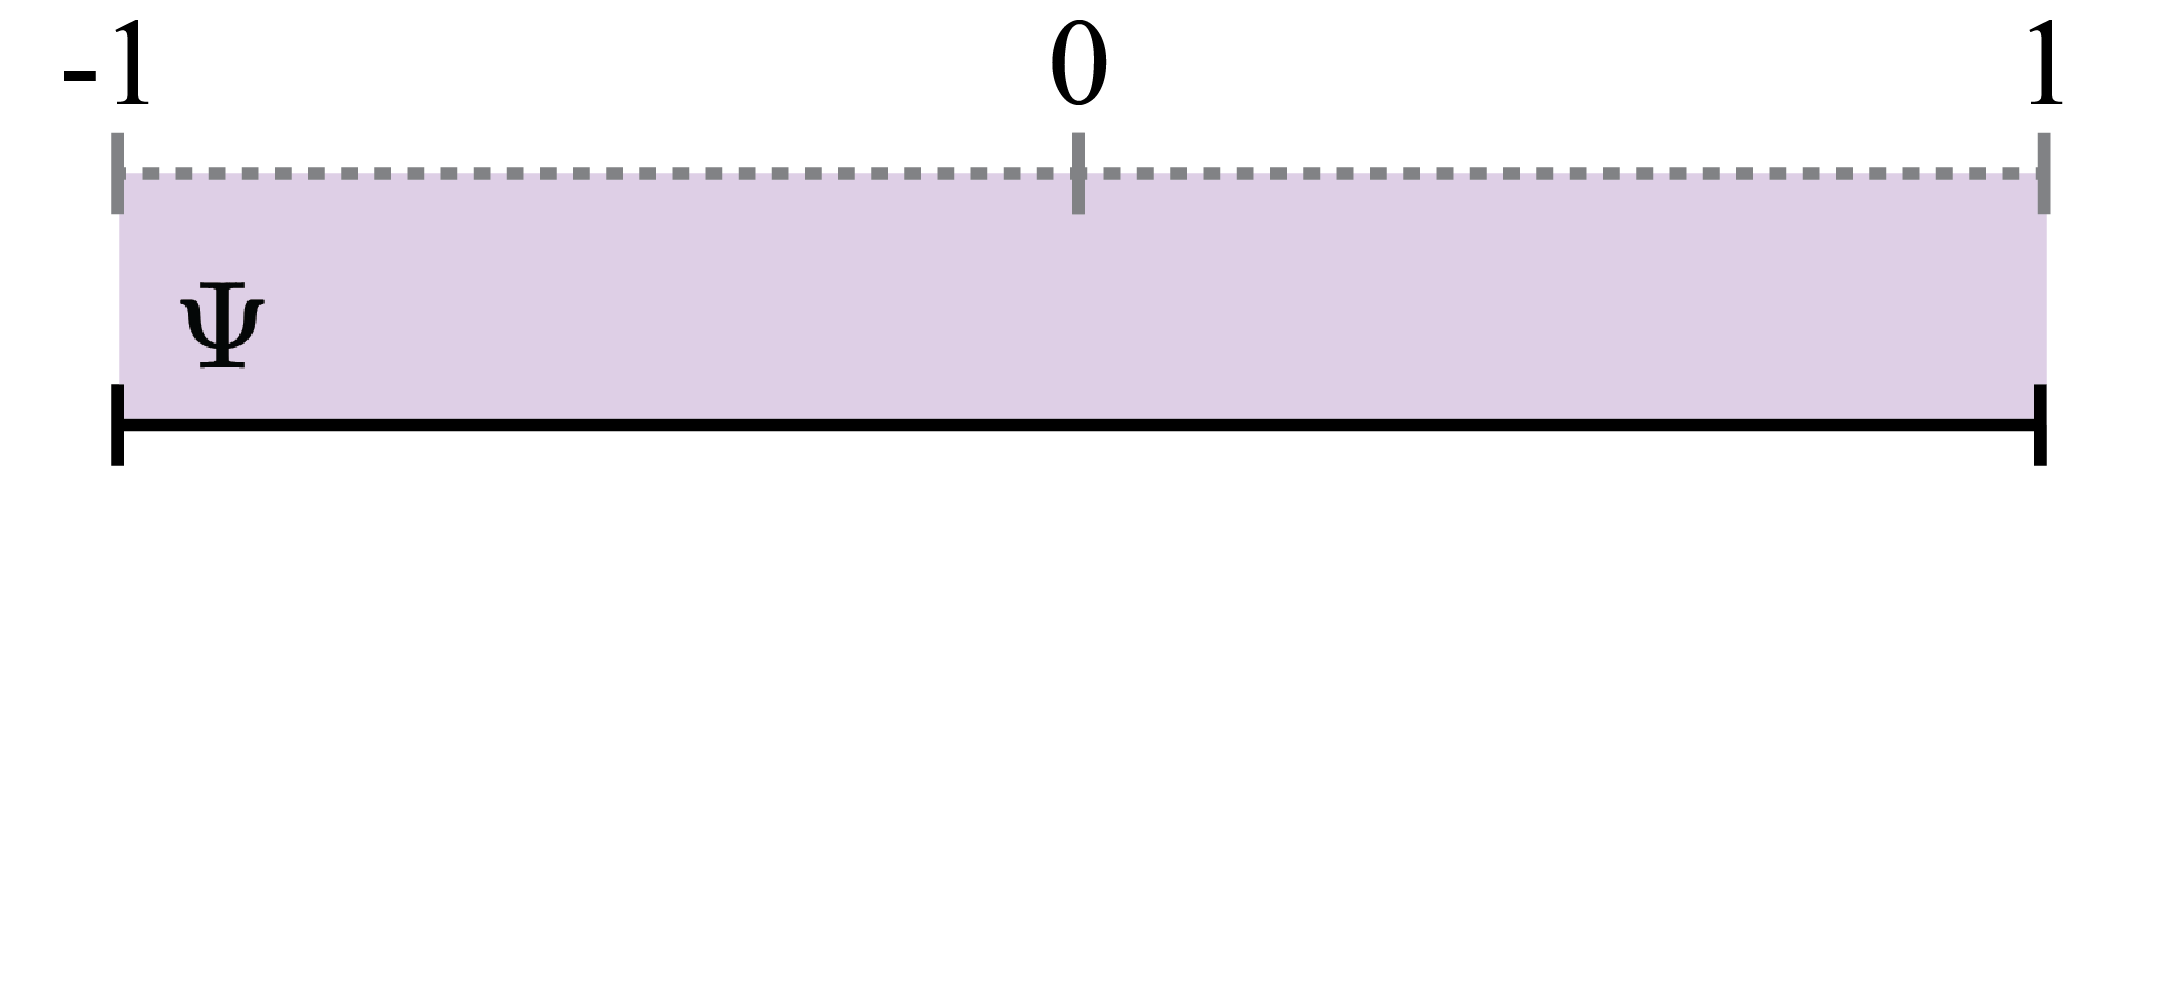
\includegraphics[width=0.90\linewidth]{images/bound1.png}
	\end{center}
\end{frame}

\begin{frame}{Learning about $\psi$}
	All methods seek to shrink the possible interval for the causal effect from $[-1, 1]$
	~\\~\\
	Can only learn more by making assumptions\footnote[frame]{``[T]he questions that we raise and our doubts depend on the fact that some propositions are exempt from doubt, are as it were like hinges on which those turn. [...] If I want the door to turn, the hinges must stay put" - Ludwig Wittgenstein \textit{On Certainty} \S 341-343}
	~\\~\\
	\textbf{Identification}: expression of causal parameter as a function of available information
	\begin{itemize}
		\item Clarifies the additional assumptions being made
	\end{itemize}
\end{frame}

\section{A Short Review of Identification with Statistical Modeling}

\begin{frame}{Setup}
	Statistical modeling would begin with collection some observations
	\begin{itemize}
		\item Data $O_i = (W_i, A_i, Y_i)$ from $n$ observations
	\end{itemize}
	~\\
	What can we learn from these observations?
	\begin{itemize}
		\item Depends on our assumptions
	\end{itemize}
\end{frame}

\begin{frame}{Some Starting Identification Assumptions}
	Assume
	\begin{itemize}
		\item[1.] \textbf{Temporality}: variables occur in the following time-order $W \rightarrow A \rightarrow Y$
		\item[2.] \textbf{Independent and Identically Distributed}: random sample of $n$ units from our target population $S=1$
		\item[3.] \textbf{No Measurement Error}: all variables in $O_i$ are correctly measured for all $n$ units
		\item[4.] \textbf{Causal Consistency}: if $a := A_i$ then $Y_i^a = Y_i$, which provides a bridge or connection between the \textit{potential} outcomes and \textit{observed} outcomes\footnote[frame]{Cole \& Frangakis \textit{Epidemiology} 2009; 20(1):3-5}
	\end{itemize}
	~\\
	What can we learn under these relatively basic assumptions?
\end{frame}

\begin{frame}{Nonparametric Bounds}
	It turns out that we can learn quite a bit
	\begin{itemize}
		\item Allow us to bound the possible causal effect
		\item From $\Psi = [-1, 1]$ to a range with a width of $1$
		\begin{itemize}
			\item \textit{Halve} the set of possible values
		\end{itemize}
		\item No information needed about study design
		\begin{itemize}
			\item No discussion about confounding, parametric models, etc.
		\end{itemize}
	\end{itemize}
\end{frame}

\begin{frame}{Nonparametric Bounds}
	\begin{center}
		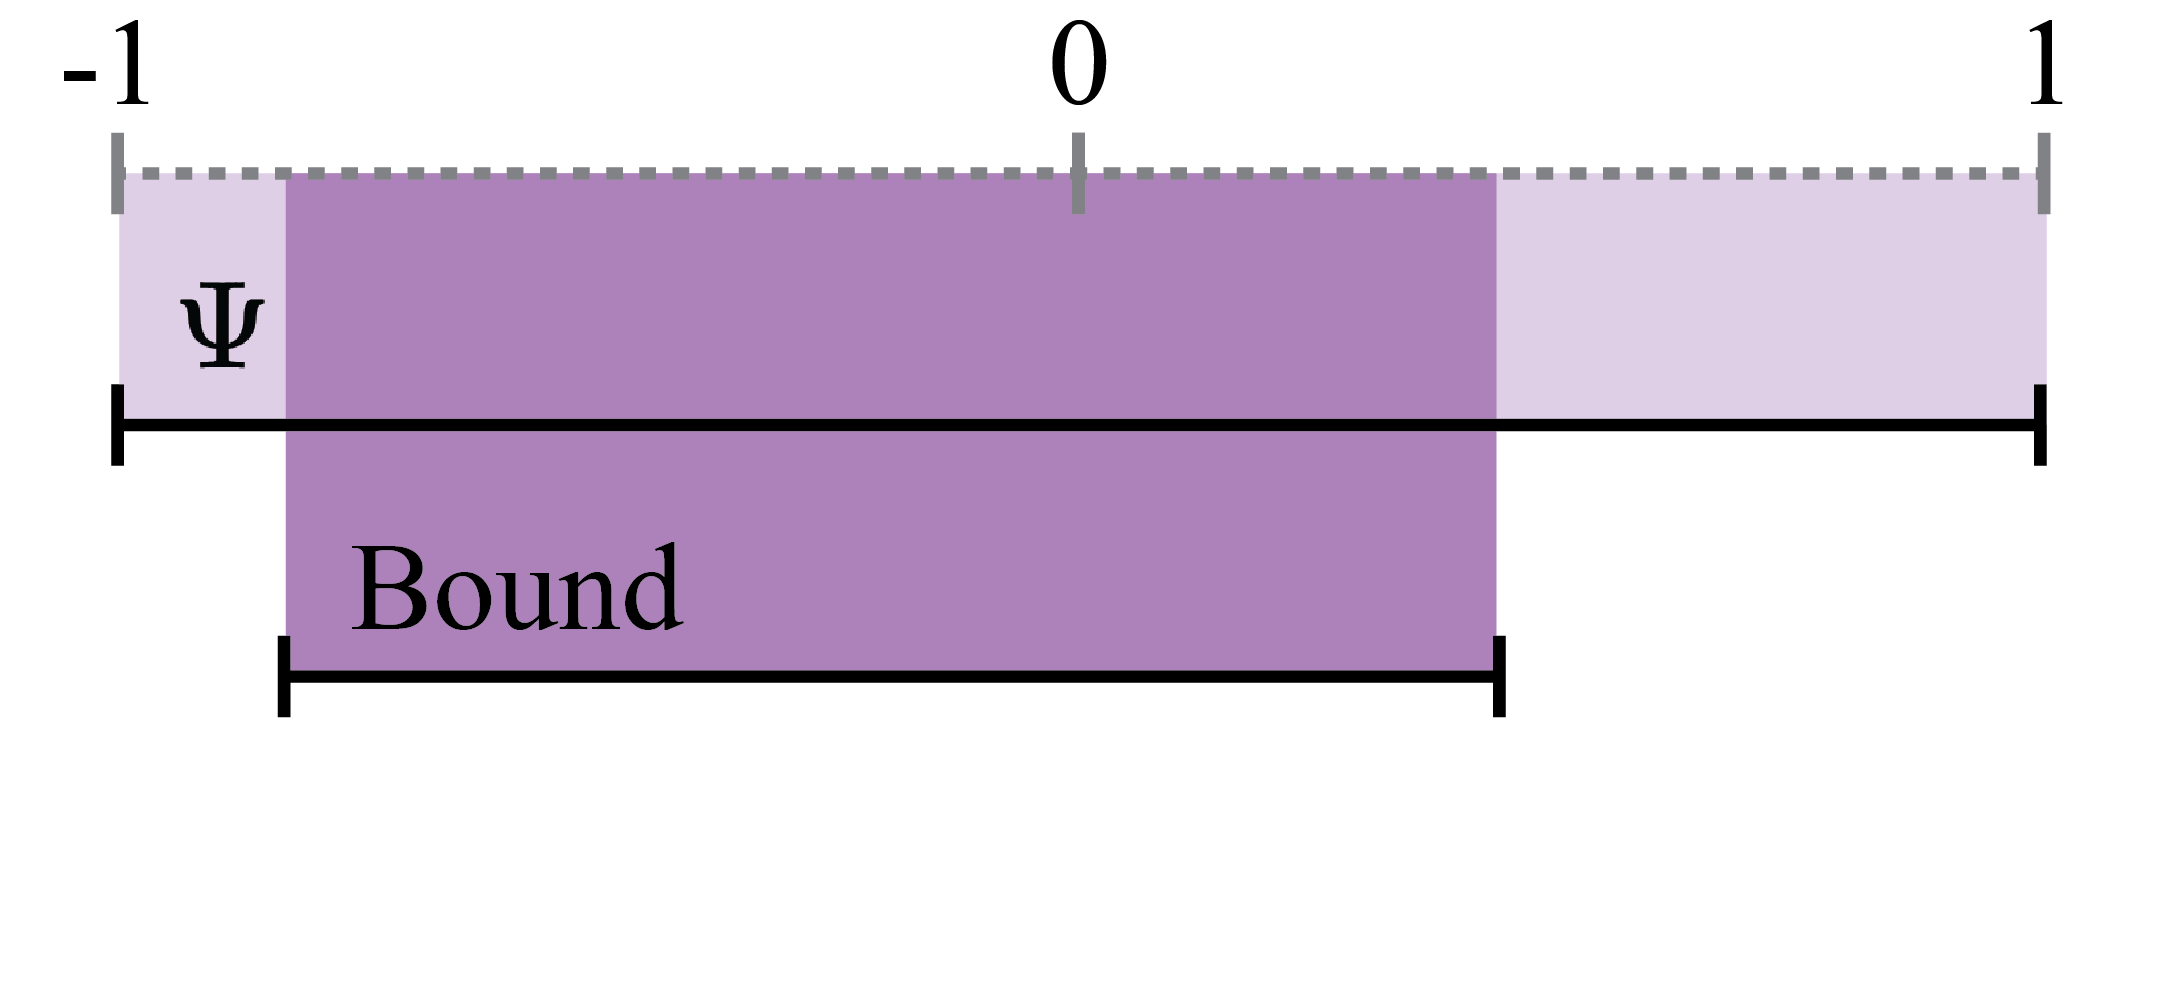
\includegraphics[width=0.90\linewidth]{images/bound2.png}
	\end{center}
\end{frame}

\begin{frame}{An Aside About Confidence Intervals}
	Bounds are distinct from Confidence Intervals (CIs).\footnote[frame]{Vansteelandt et al. \textit{Statistica Sinica} 2006; 16(3):953–979}
	\begin{itemize}
		\item Bounds capture \textit{epistemic} uncertainty
		\begin{itemize}
			\item Systematic, lack of knowledge about something
			\item Uncertainty from assumptions
		\end{itemize}
		\item CIs capture \textit{random/statistical} uncertainty
		\begin{itemize}
			\item Fluctuations due to random sampling
			\item Uncertainty from noise
		\end{itemize}
	\end{itemize}
	~\\
	Intuition
	\begin{itemize}
		\item Increasing sample size shrinks CIs but won't change the bound width
	\end{itemize}
\end{frame}

\begin{frame}{Moving Beyond the Bounds}
	Limitations
	\begin{itemize}
		\item Still unsatisfyingly wide, always contain $\psi = 0$, no causal effect
	\end{itemize}
	~\\
	To narrow the bounds, need additional assumptions
	\begin{itemize}
		\item Marginal exchangeability of $A$ and $Y^a$
		\begin{itemize}
			\item Randomized trial
		\end{itemize}
		\item Conditional exchangeability of $A$ and $Y^a$ given $W$
		\begin{itemize}
			\item Observational, no unmeasured confounding
		\end{itemize}
		\item An instrumental variable $Z$
		\item Others (e.g., proxy variables for an unmeasured confounder)
	\end{itemize}
	~\\
	These auxiliary assumptions allow us to identify a unique \textit{point}
\end{frame}

\begin{frame}{Partial and Point Identification}
	\begin{center}
		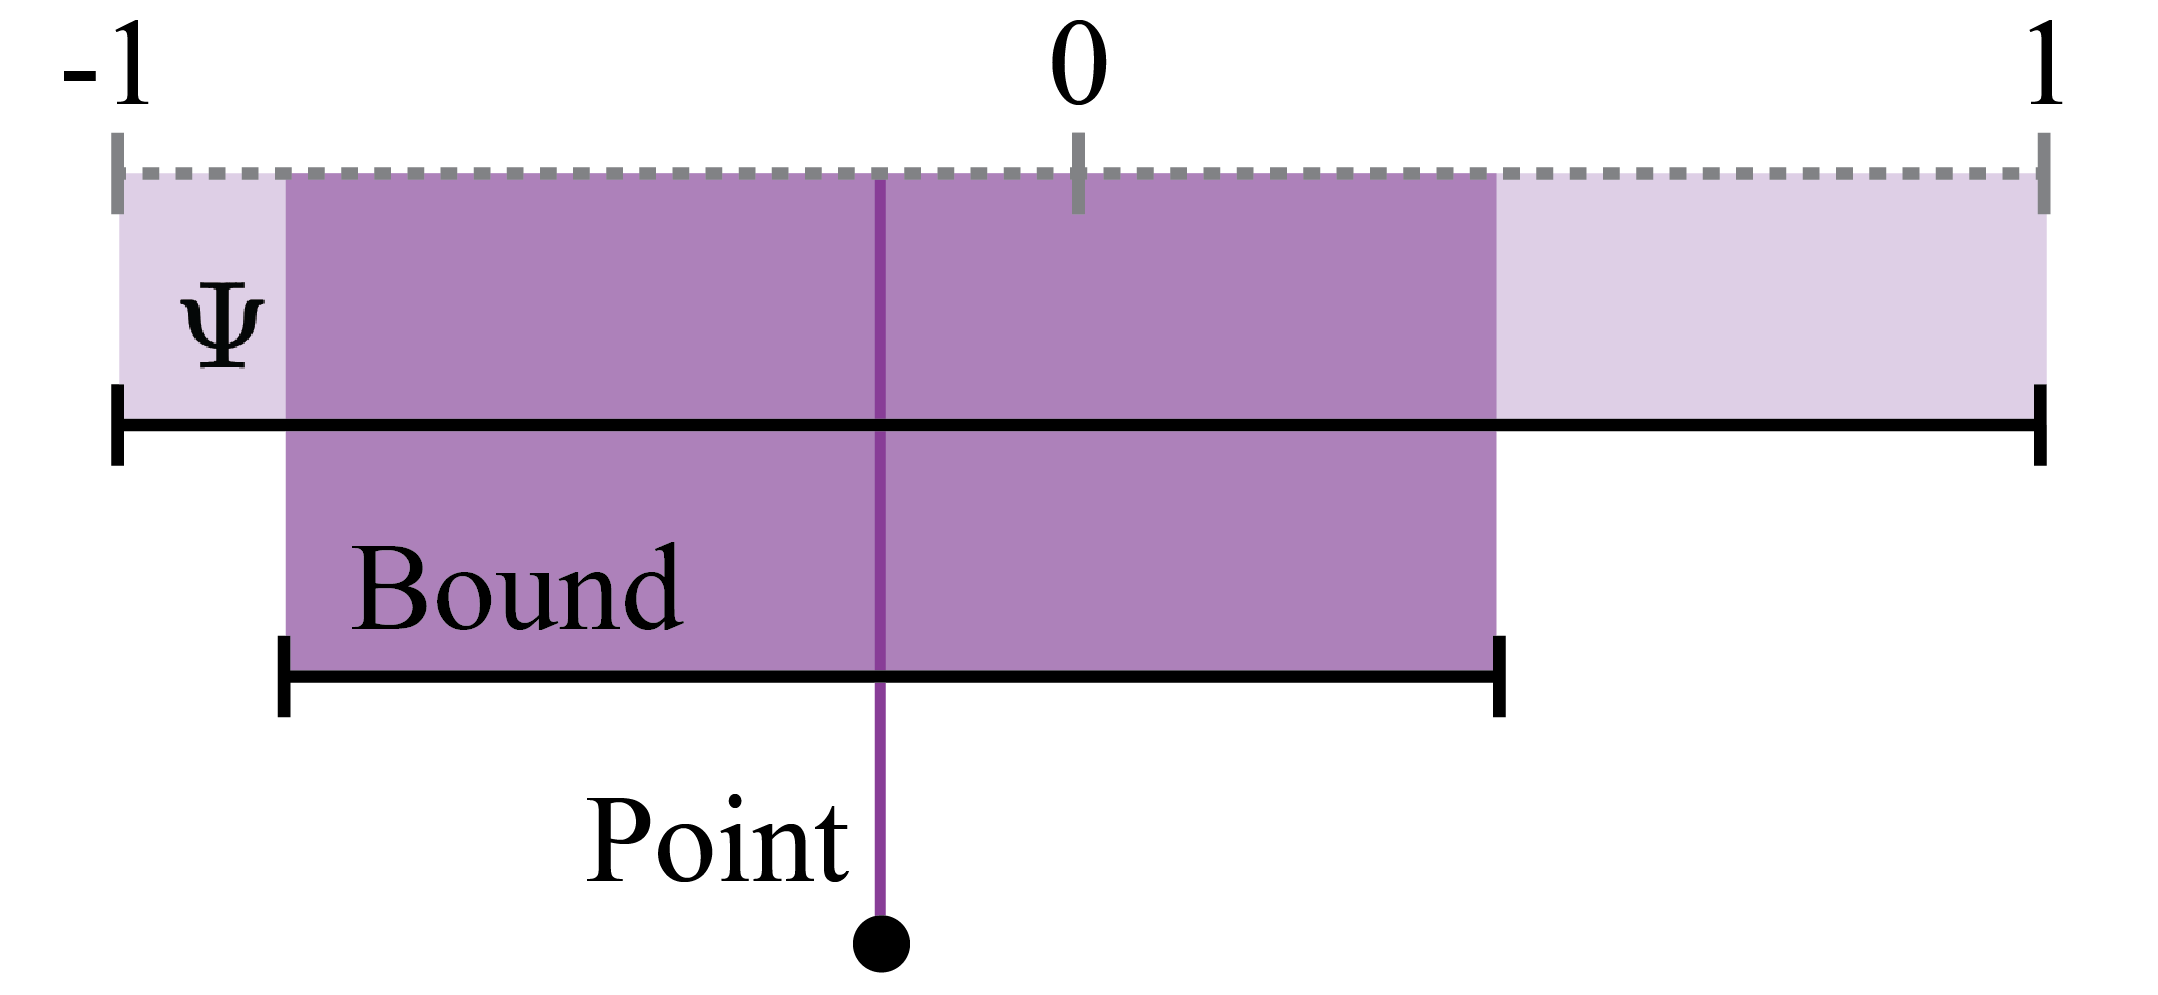
\includegraphics[width=0.90\linewidth]{images/bound3.png}
	\end{center}
\end{frame}

\begin{frame}{Example of Point Identification}
	If we also assume (or know) that 
	\begin{itemize}
		\item[5.] \textbf{Study Design}: data $O_i$ came from an observational study 
		\item[6.] \textbf{No unmeasured confounding}: $W_i$ is a sufficient adjustment set\footnote[frame]{More formally, $Y^a \amalg A \mid W$ and $0 < \Pr(A=a \mid W=w) < 1$ for all $w \in \mathcal{W}$}
	\end{itemize}
	~\\
	Then the causal effect can be point identified via
	\begin{equation*}
		\Pr_{S=1}(Y^a = 1) = \sum_{w \in \mathcal{W}} \Pr_{S=1}(Y=1 \mid A=a, W=w) \Pr_{S=1}(W=w)
	\end{equation*}
\end{frame}

\section{Extending Identification to Mathematical Models}

\begin{frame}{Setup}
	Mathematical modeling would begin with specifying a mechanism
	\begin{itemize}
		\item Base this mechanism on `theory'
		\item No directly observed data is required
	\end{itemize}
	~\\~\\
	For exposition, consider simple mechanistic model\footnote[frame]{Note that this structure implies \textbf{temporality} and \textbf{no measurement error}}
	\begin{center}
		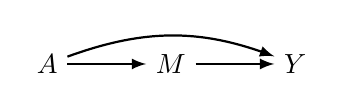
\begin{tikzpicture}
			\node (1) {$A$};
			\node [right =of 1] (2) {$M$};
			\node [right =of 2] (3) {$Y$};
			
			\draw[Arrow] (1.east) -- (2.west);
			\draw[Arrow] (2.east) -- (3.west);
			\draw[Arrow] (1) to [out=20, in=160] (3); 
		\end{tikzpicture}
	\end{center}
	\begin{itemize}
		\item For ease, suppose all binary variables
	\end{itemize}
\end{frame}

\begin{frame}{Interest Parameter}
	Remains the causal risk difference, $\psi$, but different decomposition based on mechanism
	~\\~\\
	\begin{equation*}
		\eqnmarkbox[blue]{node0}{\Pr_{S=1}(Y^a = 1)} = \sum_{m \in \{0, 1\}} \eqnmarkbox[darkgreen]{node1}{\Pr_{S=1}(Y^a = 1 \mid M^a = m)} \eqnmarkbox[violet]{node2}{\Pr_{S=1}(M^a = m)}
	\end{equation*}
	\annotate[yshift=0.7em]{right}{node0}{Parameter}
	\annotate[yshift=-0.5em]{below,left}{node1}{Probability of outcome $Y$ given $A$ and $M$}
	\annotate[yshift=0.7em]{left}{node2}{Probability of intermediate $M$ given $A$}
	~\\~\\
	These represent the \textit{true} probability functions
\end{frame}

\begin{frame}{Using a Mathematical Model}
	We specify some parameterized functions for the mechanism
	~\\~\\
	\begin{equation*}
		\eqnmarkbox[blue]{nodeM}{\bar{\psi}(\theta, \lambda)} := \sum_{m \in \{0, 1\}} \eqnmarkbox[darkgreen]{nodeH}{h(a,m; \lambda)} \eqnmarkbox[violet]{nodeG}{g(a; \theta)}
	\end{equation*}
	\annotate[yshift=0.5em]{left}{nodeM}{Math model for $\psi$}
	\annotate[yshift=0.5em]{right}{nodeH}{Function for outcome $Y$ given $A$ and $M$}
	\annotate[yshift=-1.0em]{below, left}{nodeG}{Function for intermediate $M$ given $A$}
	~\\~\\~\\
	\textbf{Identification}: assumptions that relate the chosen functions and their parameters, $(\theta, \lambda)$, to the true probabilities
\end{frame}

\begin{frame}{Identification}
	The assumed structure already has \textbf{temporality} and \textbf{measurement error} built in
	~\\~\\
	Some additional restrictions on $h$ and $g$
	\begin{itemize}
		\item[1.] Both functions return values in $[0,1]$ for parameter spaces $\Theta,\Lambda$.\footnote[frame]{Formally, $g:\Theta \rightarrow [0,1]$, $h:\Lambda \rightarrow [0,1]$}
		\item[2.] Output of $g$ ($h$) covers $[0,1]$ for all unique values of $a$ (and $m$) for $\Theta$ ($\Lambda$)\footnote[frame]{Formally, $\{g(a; \theta) : \theta \in \Theta \} = [0,1]$, $\{h(a, m; \lambda) : \lambda \in \Lambda \} = [0,1]$ for all unique values of $a,m$}
	\end{itemize}
	~\\
	Why: ensures that $\bar{\psi}(\theta, \lambda)$ covers all of $\Psi$ for valid parameters
	\begin{itemize}
		\item Ruling out possible $\psi$ values is done through choices of $\theta,\lambda$, not $g,h$
		\item Call math models that meet this property \textit{vacuous} models
	\end{itemize}
\end{frame}

\begin{frame}{Vacuous vs Non-vacuous Models}
	\begin{center}
		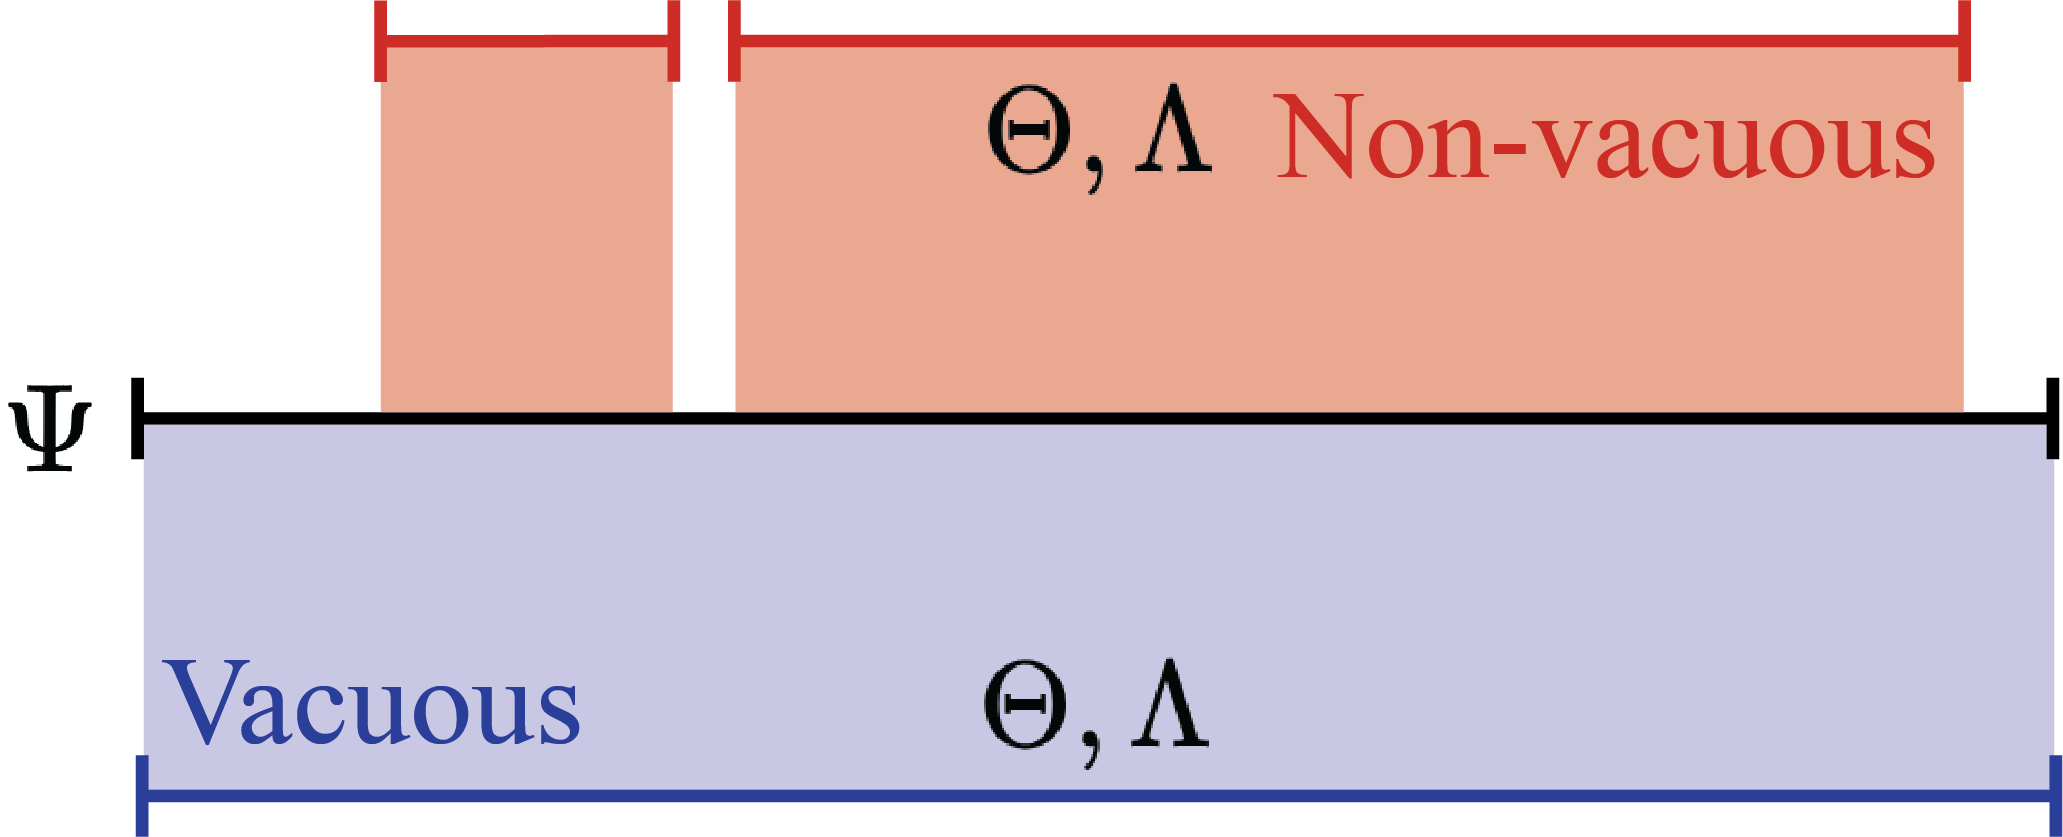
\includegraphics[width=0.95\linewidth]{images/bounds_vacuous.png}
	\end{center}
\end{frame}

\begin{frame}{Point Identification}
	Now we simply have to select values of $\theta,\lambda$
	~\\~\\ 
	Given $h,g$, suppose we could ask an oracle\footnote[frame]{or genie, or sphinx, or your favorite other mythical being with magic insight} to reveal the correct (true) parameter choices for these functions, denoted as $\theta^*,\lambda^*$. Then for all unique $a,m$
	\begin{equation*}
		\begin{aligned}
			g(a; \theta^*) = & \Pr_{S=1}(M^a = 1) \\
			h(a,m; \lambda^*) = & \Pr_{S=1}(Y^a = 1 \mid M^a = m)
		\end{aligned}
	\end{equation*}
	~\\
	Then it follows that $\psi = \bar{\psi}(\theta^*, \lambda^*)$
	\begin{itemize}
		\item A \textit{vacuous} model ensures $\theta^*,\lambda^*$ exist
	\end{itemize}
\end{frame}

\begin{frame}{Partial Identification}
	Knowledge of $\theta^*,\lambda^*$ is difficult.\footnote[frame]{If not unreasonable outside the world of examples we can create} Consider partial identification instead
	\begin{itemize}
		\item Subset of possible values for $\theta^*$, denoted by $\Theta^*$
		\item Subset of possible values for $\lambda^*$, denoted by $\Lambda^*$ 
	\end{itemize}
	~\\
	\textbf{Model Capture}: for all unique $a,m$ assume that
	~\\~\\
	\begin{equation*}
		\eqnmarkbox[blue]{nodeT}{\Pr_{S=1}(M^a = 1)} 
		\eqnmarkbox[black]{nodeI}{\in} 
		\eqnmarkbox[red]{nodeO}{\{g(a; \theta) : \theta \in \Theta^*\}}
	\end{equation*}
	\annotate[yshift=0.5em]{left}{nodeT}{True probability}
	\annotate[yshift=-0.5em]{below,left}{nodeI}{is within the}
	\annotate[yshift=0.5em]{right}{nodeO}{possible outputs for function}	
	~\\
	\begin{equation*}
		\eqnmarkbox[blue]{nodeU1}{\Pr_{S=1}(Y^a = 1 \mid M^a = m)} 
		\eqnmarkbox[black]{nodeU2}{\in} 
		\eqnmarkbox[red]{nodeU3}{\{h(a, m; \lambda) : \lambda \in \Lambda^*\}}
	\end{equation*}
\end{frame}

\begin{frame}{Alternative Expression}
	Another (maybe easier) way to specify the \textbf{Model Capture} assumption
	~\\~\\
	\begin{equation*}
		\eqnmarkbox[blue]{nodeT}{\theta^*} 
		\eqnmarkbox[black]{nodeI}{\in} 
		\eqnmarkbox[red]{nodeO}{\Theta^*}
	\end{equation*}
	\annotate[yshift=0.5em]{left}{nodeT}{True parameter}
	\annotate[yshift=-0.5em]{below,left}{nodeI}{is within the}
	\annotate[yshift=0.5em]{right}{nodeO}{set of considered values}	
	~\\
	\begin{equation*}
		\eqnmarkbox[blue]{nodeU1}{\lambda^*} 
		\eqnmarkbox[black]{nodeU2}{\in} 
		\eqnmarkbox[red]{nodeU3}{\Lambda^*}
	\end{equation*}
\end{frame}

\begin{frame}{Partial Identification}
	\textbf{Model Capture} allows for
	~\\~\\
	\begin{equation*}
		\eqnmarkbox[green]{nodeP}{\psi} 
		\eqnmarkbox[black]{nodeI}{\in} 
		\eqnmarkbox[darkblue]{nodeM}{\left\{ \bar{\psi}(\theta, \lambda) : \theta, \lambda \in \Theta^* \times \Lambda^* \right\} = \Psi^*}
		\eqnmarkbox[black]{nodeW}{\subset}
		\eqnmarkbox[darkgreen]{nodeS}{\Psi}
	\end{equation*}
	\annotate[yshift=0.5em]{left}{nodeP}{True parameter}
	\annotate[yshift=0.5em]{right}{nodeI}{is within the}
	\annotate[yshift=0.5em]{right}{nodeM}{possible outputs of the math model}	
	\annotate[yshift=-0.5em]{below,left}{nodeW}{which is smaller than}	
	\annotate[yshift=-0.5em]{below,right}{nodeS}{parameter space}	
	~\\~\\~\\
	In other words, we can compute bounds for $\psi$
\end{frame}

\begin{frame}{Identification Visualization}
	\begin{center}
		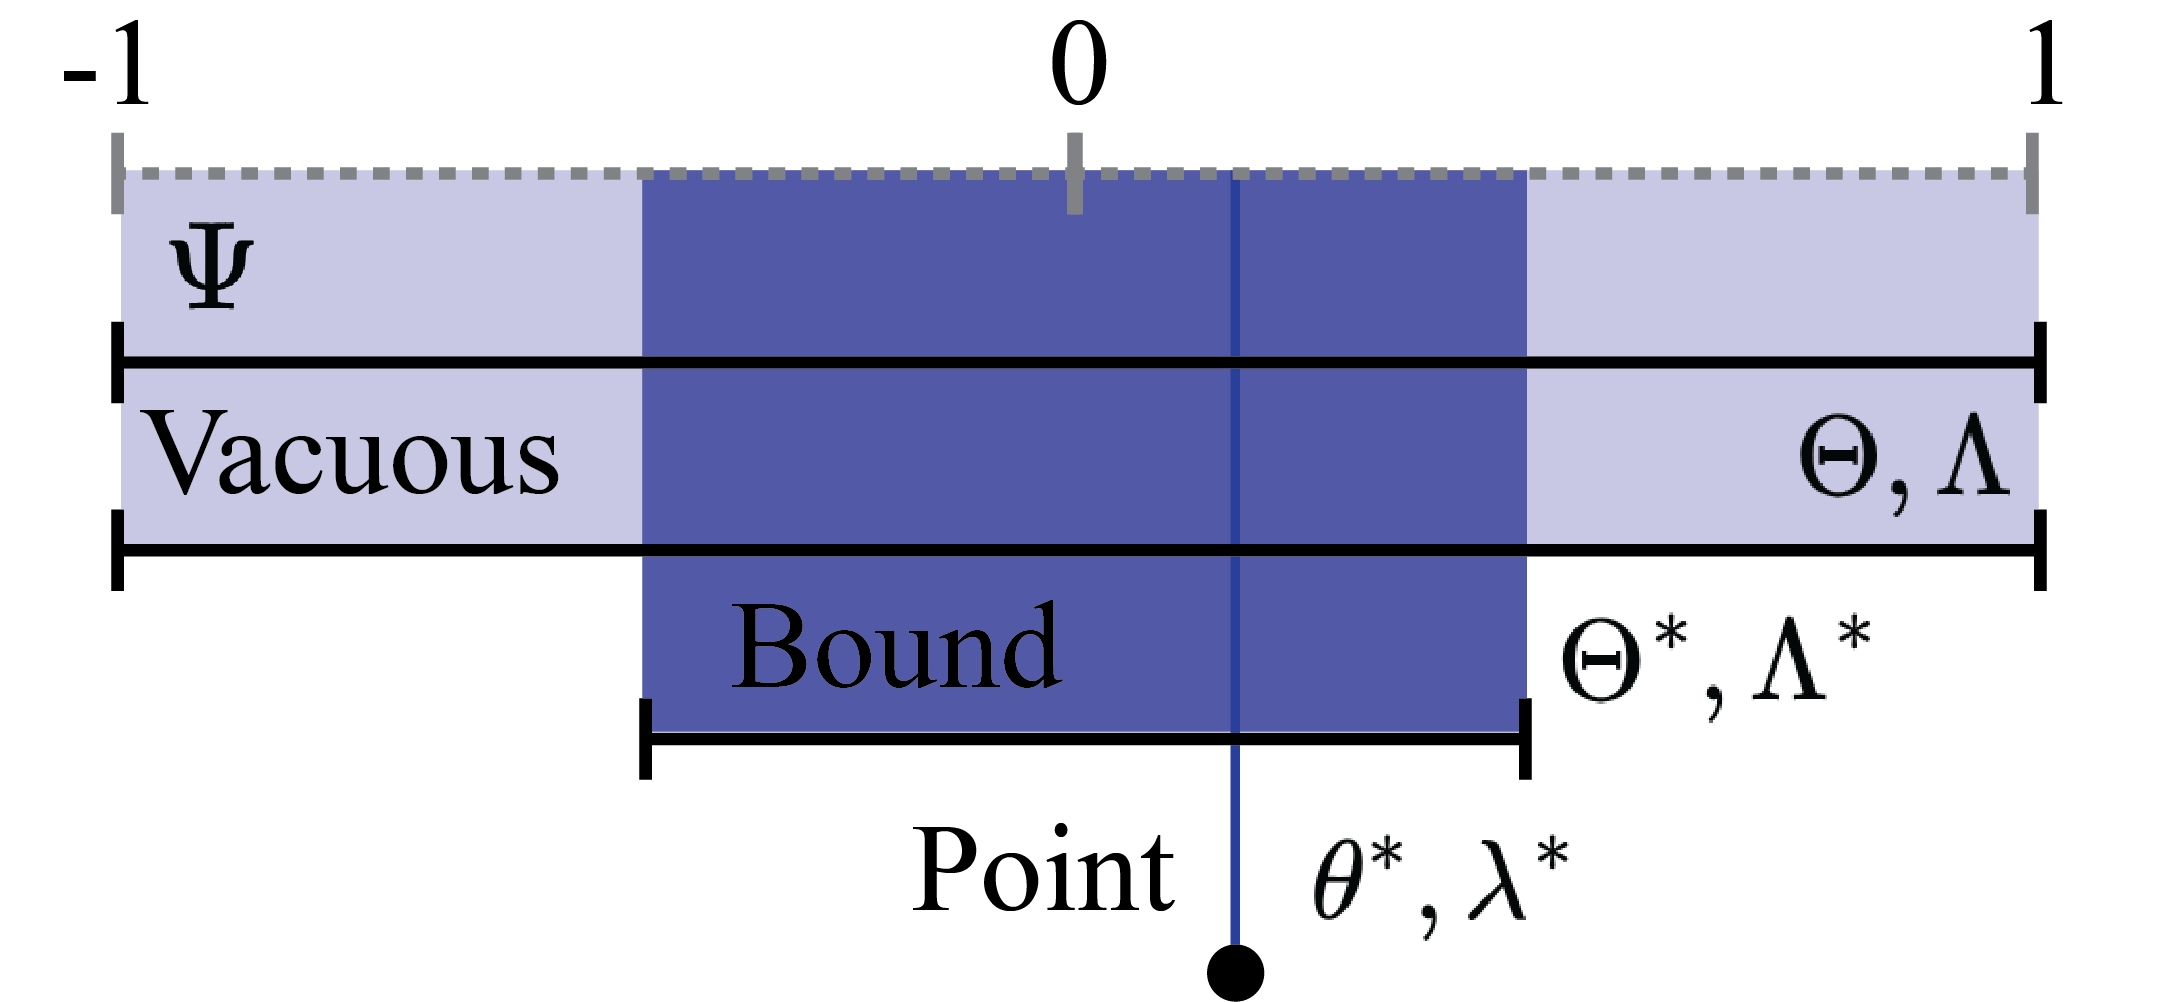
\includegraphics[width=0.90\linewidth]{images/bounds_math.png}
	\end{center}
\end{frame}

\begin{frame}{Some Implications}
	Vacuous model
	\begin{itemize}
		\item Ought to prefer vacuous models when we can construct them
		\item Analogous to parametric vs nonparametric identification in statistical modeling\footnote[frame]{The g-null paradox for the g-formula is one such example} 
	\end{itemize}
	~\\
	Width of mathematical model bounds
	\begin{itemize}
		\item Function of choices for $\Theta^*, \Lambda^*$
		\item Unlike statistical modeling, no guaranteed size reduction in bounds
		\item Like statistical modeling, information needs to be relevant for $S=1$		
	\end{itemize}
\end{frame}

\section{Motivating Example}

\begin{frame}{Pharmacoepidemiology Example}
	\textbf{Question}: effect of amlodipine (10 mg)\footnote[frame]{A calcium channel blocker used to treat high blood pressure and chest pain} vs placebo on hypertension status at 24 hours?
	\begin{itemize}
		\item Population: adults with a SBP $\ge 140$ in the US
	\end{itemize}
	~\\
	\textbf{Notation}
	\begin{itemize}
		\item $A$: treatment (1: amlodipine, 0: placebo)
		\item $Y$: hypertension status\footnote[frame]{Defined as a systolic blood pressure of $\ge 140$ mm Hg} 24 hours after baseline
		\item $S=1$: US adults with a SBP $\ge 140$
		\item $\psi$: corresponding causal risk difference
	\end{itemize}
\end{frame}

\begin{frame}{Statistical Modeling}
	Can learn $\psi$ by
	\begin{itemize}
		\item Conducting a randomized trial
		\item Use existing observational data and rely on some unverifiable assumptions (e.g., no unmeasured confounding)
		\item Rely on only the bounds
	\end{itemize}
	~\\
	Regardless of approach taken, identification allows us to more clearly articulate assumptions
\end{frame}

\begin{frame}{Mathematical Modeling}
	No direct observations on $(A,Y)$ and instead rely on theory
	\begin{itemize}
		\item External information or beliefs about amlodipine and SBP
	\end{itemize}
	~\\
	Assume structure between different variables
	\begin{center}
		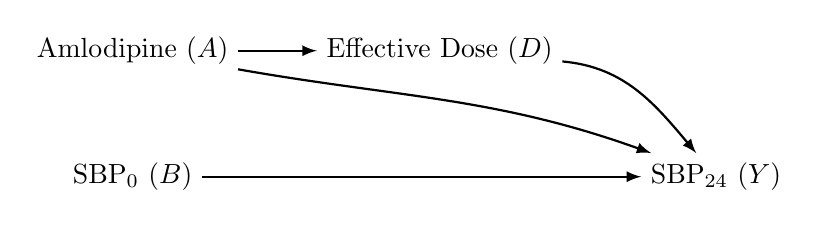
\begin{tikzpicture}
			\node (1) {SBP\textsubscript{0} ($B$)};
			\node [above =of 1] (2) {Amlodipine ($A$)};
			\node [right =of 2] (3) {Effective Dose ($D$)};
			\node [below right =of 3] (4) {SBP\textsubscript{24} ($Y$)};
			
			\draw[Arrow] (1.east) -- (4.west);
			\draw[Arrow] (2.east) -- (3.west);
			\draw[Arrow] (3) to [out=-5, in=130] (4); 
			\draw[Arrow] (2) to [out=-10, in=160] (4); 
		\end{tikzpicture}
	\end{center}
\end{frame}

\begin{frame}{Mathematical Modeling}
	Pharmacodynamic model
	\begin{equation*}
		\bar{\psi}(\gamma, \theta, \lambda) = 
		\int_{\mathcal{B}} 
		\eqnmarkbox[redorange]{nodeh}{h(b, a, \eqnmarkbox[cyan]{nodeg}{g(a, \theta)}; \lambda)}
		\eqnmarkbox[violet]{nodef}{f(b; \gamma)}
	\end{equation*}
	~\\
	{\color{violet} Probability density function for blood pressure}, $\gamma$
	\begin{itemize}
		\item Determined by the population
	\end{itemize}
	{\color{cyan} Function for effective dose}, $\theta$
	\begin{itemize}
		\item Active drug bioavailable at 24 hours given $a$
	\end{itemize}
	{\color{redorange} Function for hypertension status}, $\lambda$
	\begin{itemize}
		\item Return hypertension given $b,a,d$
	\end{itemize}
\end{frame}

\begin{frame}{Mathematical Model Components}
		\begin{columns}
		\begin{column}{0.7\textwidth}
			$\eqnmarkbox[violet]{nodef}{f(b; \gamma)}$ -- Probability density function for blood pressure
			\begin{itemize}
				\item Leave as generic probability density function
				\item \textbf{External Information}: Need SBP for US adults with SBP $>140$
				\begin{itemize}
					\item $\gamma$ based on empirical distribution of the first measured SBP from NHANES\footnote[frame]{National Health and Nutrition Survey} 2017-2018
				\end{itemize}
			\end{itemize}
		\end{column}
		\begin{column}{0.3\textwidth}
			\begin{center}
				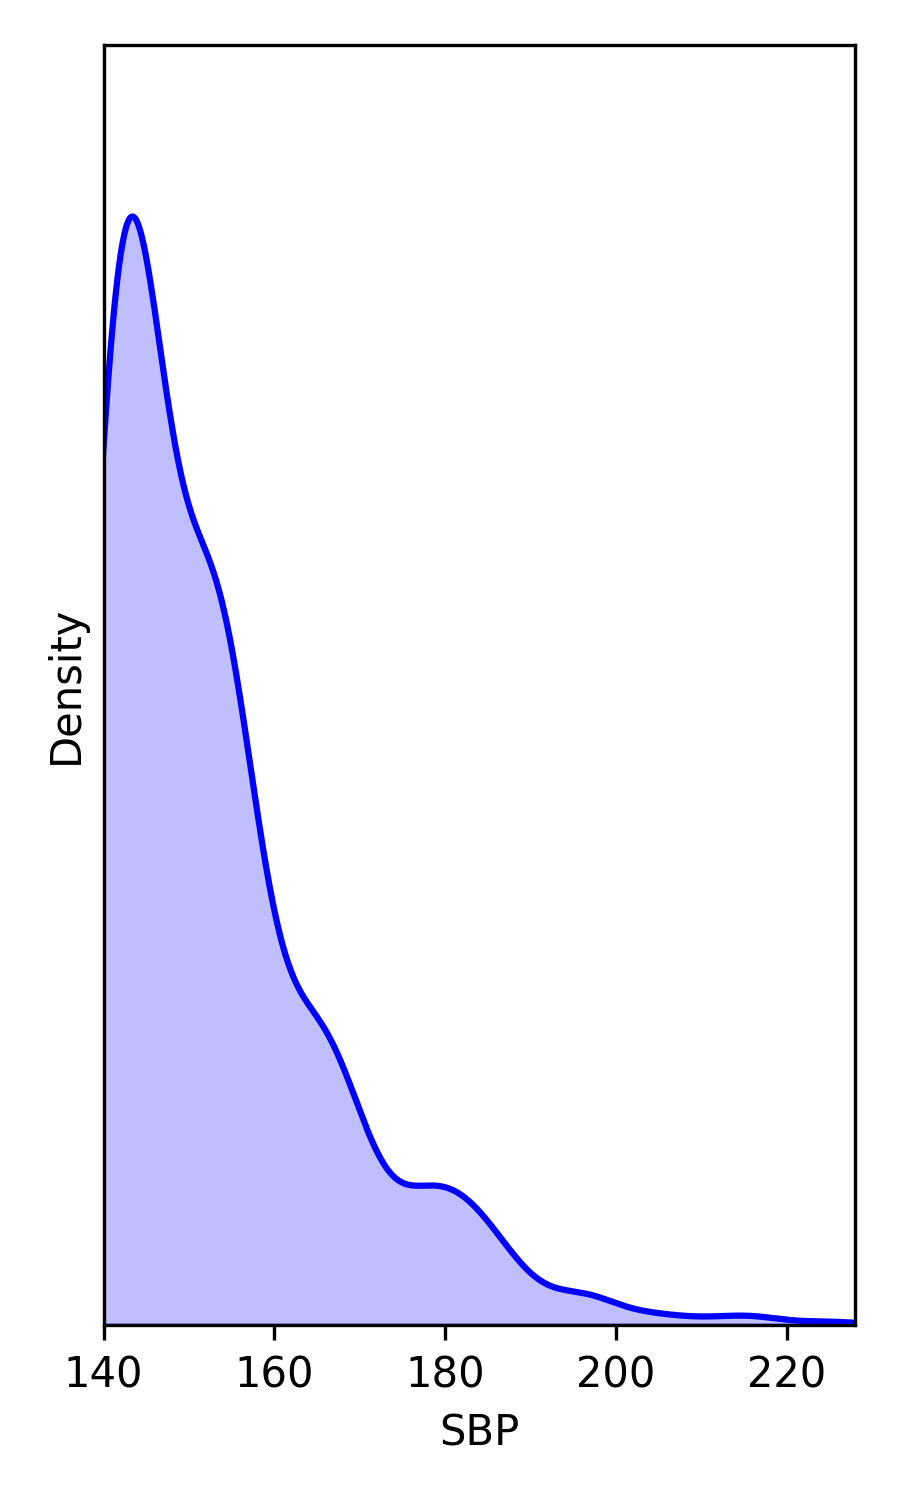
\includegraphics[width=0.95\linewidth]{images/sbp_density.png}
			\end{center}
		\end{column}
	\end{columns}	
\end{frame}

\begin{frame}{Mathematical Model Components}
	$\eqnmarkbox[cyan]{nodef}{g(a; \theta)}$ -- effective dose
	\begin{itemize}
		\item Simple proportion model: $g(a,\theta) = \theta_0 \times \theta_1$
		\begin{itemize}
			\item $\theta_0$: dose of amlodipine, $\theta_1$: percent of available drug at 24 hours
			\item Non-negative values will always return non-negative effective dose
		\end{itemize}
		\item \textbf{External Information}: 
		\begin{itemize}
			\item $\theta_0 = 10$ when $A=1$ and zero otherwise
			\item $\Theta_1^* = [25\%, 40\%]$ based on dosing study\footnote[frame]{Kim et al. \textit{Clinical Therapeutics} 2013; 35(7):934-940}
		\end{itemize}
	\end{itemize}
\end{frame}

\begin{frame}{Mathematical Model Components}
	$\eqnmarkbox[redorange]{nodef}{h(b,a,m;\lambda)}$ -- hypertension status
	\begin{itemize}
		\item $h(b,a,m;\lambda) = I\left(\bar{y}(b,a,m; \lambda) < 140\right)$, with E-max model
	\end{itemize}
	\begin{equation*}
		\bar{y}(b,a,m; \lambda) = b - \left[ \lambda_0 + a \lambda_1 \left( \frac{m}{\lambda_2 + m} \right) + a \lambda_3 \right]
	\end{equation*}	
	~\\
	\textbf{External Information}:
	\begin{itemize}
		\item $\lambda_0$: constant change in $B$, $\lambda^*_0 := 0$
		\item $\lambda_1$: maximum response, $\Lambda^*_1 := [16.3, 36.3]$.\footnote[frame]{Park et al. \textit{ Basic Clin Pharmacol Toxicol}, 2019; 125(4):345-352}
		\item $\lambda_2$: ED50, $\Lambda^*_2 := [0.1, 13.0]$.\footnote[frame]{Heo et al. \textit{British Journal of Clinical Pharmacology} 2016; 82(6):1557-1567}
		\item $\lambda_3$: effect of amlodipine not through effective concentration, $\lambda^*_3 := 0$
	\end{itemize}
\end{frame}

\begin{frame}{Results}
	Applying the model, we get $\Psi^* = [0.23, 0.91]$
	\begin{itemize}
		\item Amlodipine is effective at reducing hypertension status 
	\end{itemize}
	\begin{center}
		
\includegraphics[width=0.8\linewidth]{images/example_results.png}
	\end{center}
	But can we trust these results
	\begin{itemize}
		\item Review the identification assumptions being made
	\end{itemize}
\end{frame}

\begin{frame}{Evaluation of the Mathematical Model}
	\textbf{Model Capture}:
	\begin{itemize}
		\item $\eqnmarkbox[violet]{nodef}{f(b; \gamma)}$
		\begin{itemize}
			\item Assumes NHANES 2017-2018 \textit{exactly }represents SBP distribution for $S=1$
		\end{itemize}
		\item $\eqnmarkbox[cyan]{nodef}{g(a; \theta)}$
		\begin{itemize}
			\item No manufacturing error with dosage
			\item Available drug info comes from male South Koreans with SBP $<150$.\footnote[frame]{Body weight distributions are also substantially different (mean: 68 kg South Korean, 84 kg NHANES)}
		\end{itemize}
		\item $\eqnmarkbox[redorange]{nodef}{h(b, a, m; \lambda)}$
		\begin{itemize}
			\item $\lambda_0 := 0$ means no natural variation in hypertension over 24 hours
			\item Choices for $\lambda_1,\lambda_2$ also comes from South Koreans with SBP $<150$
			\item $\lambda_3 := 0$ means side-effects (e.g., nausea, fatigue) do not alter behaviors
			% \item $\bar{y}$ can return negative values, so care needs to be done when selecting $\lambda$
		\end{itemize}
	\end{itemize}
	~\\
	Summary: concerns about information sources, bounds likely too narrow
\end{frame}

\section{Conclusions}

\begin{frame}{Conclusions}
	Identification provides framework to compare statistical and mathematical modeling
	\begin{itemize}
		\item Focus on bounding causal effects
		\item Help formalize assumptions and how to talk about them
		\item Opens up analogies between the two traditions
	\end{itemize}
	~\\
	Illustrated with a simple pharmacodynamic model
	\begin{itemize}
		\item Highlights issues for the model
		\item Concrete suggestions on how to improve the model
	\end{itemize}
\end{frame}

\begin{frame}{Bigger Picture}
	Provides a way to communicate across fields
	\begin{itemize}
		\item Helpful to be comfortable with both traditions for infectious disease epidemiology
		\item More holistic view of how we can address pressing scientific questions
	\end{itemize}
	~\\
	Framework allows for traditions to be jointly used to address a question
	\begin{itemize}
		\item My own work uses mathematical models for extrapolation under uncertainty with statistical models, and to address non-positivity\footnote[frame]{Zivich et al. \textit{Epidemiology} 2024; 35(1):23-31, Zivich et al. \textit{JECH} 2026; In-Press}
		\begin{itemize}
			\item Framework more clearly lays out assumptions being made
		\end{itemize}
		\item Can re-examine other hybrid models
	\end{itemize} 
\end{frame}

\begin{frame}{Future Directions}
	Extend from bounds to distributions for $\psi$
	\begin{itemize}
		\item Reflect amount of (un)certainty in information on $\theta,\lambda$
	\end{itemize}
	~\\
	Extend to allow for interactions between units
	\begin{itemize}
		\item Major use of mathematical models
		\item Can be done under an interference framework from causal inference\footnote[frame]{Hudgens \& Halloran \textit{JASA} 2008; 103(482):832-842}
	\end{itemize}
	~\\
	Actual application to build or compare mathematical models
\end{frame}

\begin{frame}{Thank You}
	\begin{center}
		\Large
		Questions?
	\end{center}
	~\\~\\
	\begin{center}
		\small
		\faEnvelope \quad pzivich@unc.edu \qquad \quad 
		\faGithub \quad pzivich \qquad \quad
		\faHashtag \quad pausalz@bsky.social
	\end{center}	
	~\\~\\
	\begin{center}
		Zivich PN \textit{arXiv:2511.01960}
	\end{center}
\end{frame}

\section{Appendix}

\begin{frame}{Constructing the Bounds}
	It follows that
	\begin{equation*}
		\begin{aligned}
			\eqnmarkbox[blue]{node1}{\Pr_{S=1}(Y^1 = 1)} & = 
			\eqnmarkbox[black]{node2}{\Pr_{S=1}(Y^1 = 1 \mid A=1) \Pr_{S=1}(A=1) + \Pr_{S=1}(Y^1 = 1 \mid A=0)\Pr_{S=1}(A=0)} \\
			& = \eqnmarkbox[black]{node3}{\Pr_{S=1}(Y = 1 \mid A=1)} \Pr_{S=1}(A=1) + \Pr_{S=1}(Y^1 = 1 \mid A=0)\Pr_{S=1}(A=0)
		\end{aligned}
	\end{equation*}
	\annotate[yshift=0.7em]{right}{node2}{Law of total probability}
	\annotate[yshift=-0.5em]{below,right}{node3}{Causal consistency}
	~\\~\\~\\
	All quantities in terms of $O_i$, except $\Pr_{S=1}(Y^1 = 1 \mid A=0)$
	\begin{itemize}
		\item But we know it must be within $[0,1]$
	\end{itemize}
\end{frame}

\begin{frame}{Synthesis: Case Study in Transportability}
	Trial on impact of 2- vs 1-drug therapy on 20-week CD4 (marker of disease progression) in women with HIV\footnote[frame]{Case study from Zivich et al. \textit{J R Stat Soc Series A} 2025; 188(1):158-180}
	\begin{itemize}
		\item Average causal effect comparing 2- vs 1-drug on 20-week CD4 in target population
		\item ACTG 175 (trial) and WIHS (sample of target population)
	\end{itemize}
	~\\
	To transport assume populations are exchangeable given
	\begin{itemize}
		\item Baseline CD4\footnote[frame]{This analysis also accounts for age, race, weight. Positivity was assumed for these variables}
	\end{itemize}
\end{frame}

\begin{frame}{Distribution of Baseline CD4}
	\begin{center}
		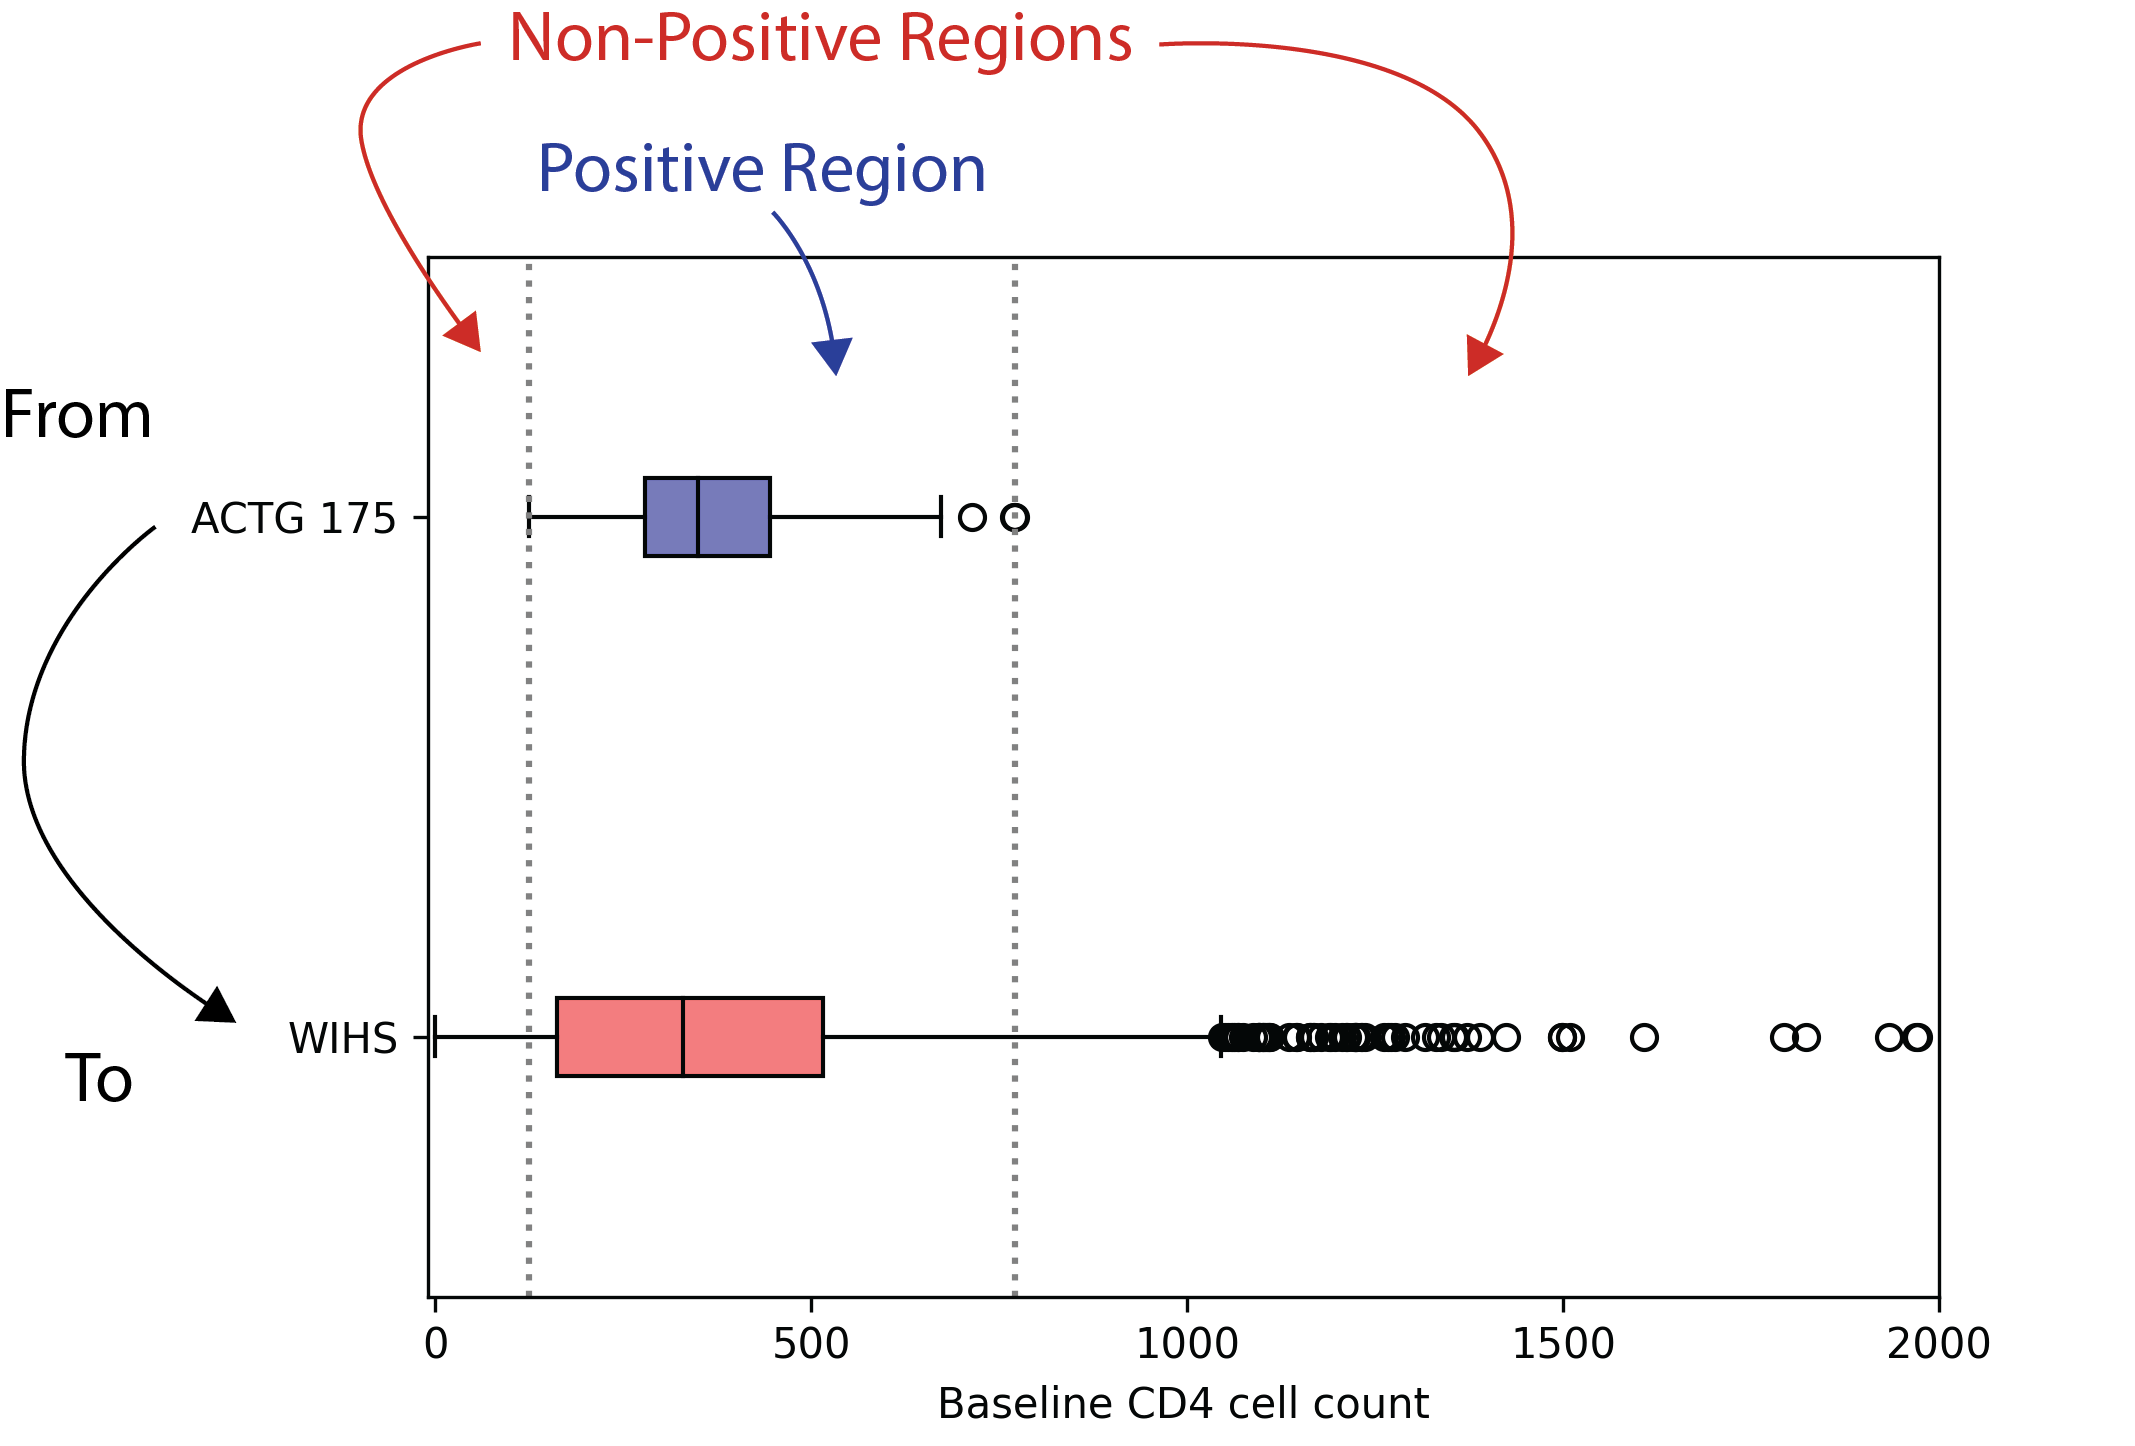
\includegraphics[width=0.75\linewidth]{images/pop_density_annotated.png}	
	\end{center}
\end{frame}

\begin{frame}{Re-Expression of the Parameter}
	\begin{equation*}
		\psi = \eqnmarkbox[darkblue]{node1}{E[Y^1 - Y^0 \mid S=1]}
		= 
		E\left\{ 
		\eqnmarkbox[darkred]{node0}{E[Y^1 - Y^0 \mid V, S=1]}
		\mid S=1 \right\}
	\end{equation*}
	\annotate[yshift=0.6em]{above,right}{node1}{Average causal effect (ACE) in population $S=1$}	
	\annotate[yshift=-0.6em]{below,left}{node0}{Conditional average causal effect (CACE) by $V$}	
	~\\~\\
	... or that the ACE is the CACE marginalized over the distribution of baseline CD4 values (i.e., $V$) in the target population (i.e., $S=1$)\footnote[frame]{Where $Y^a$ is the potential outcome under $a$ and $E[\cdot]$ is the expected value function}
	~\\~\\
	Therefore, we can look at the {\color{darkred}CACE} for intuition on how non-positivity by $V$ impacts estimation of the {\color{darkblue}ACE}\footnote[frame]{For estimation of the CACE, I used an augmented inverse probability weighting estimator}
\end{frame}

\begin{frame}{Conditional Average Causal Effect}
	\begin{center}
		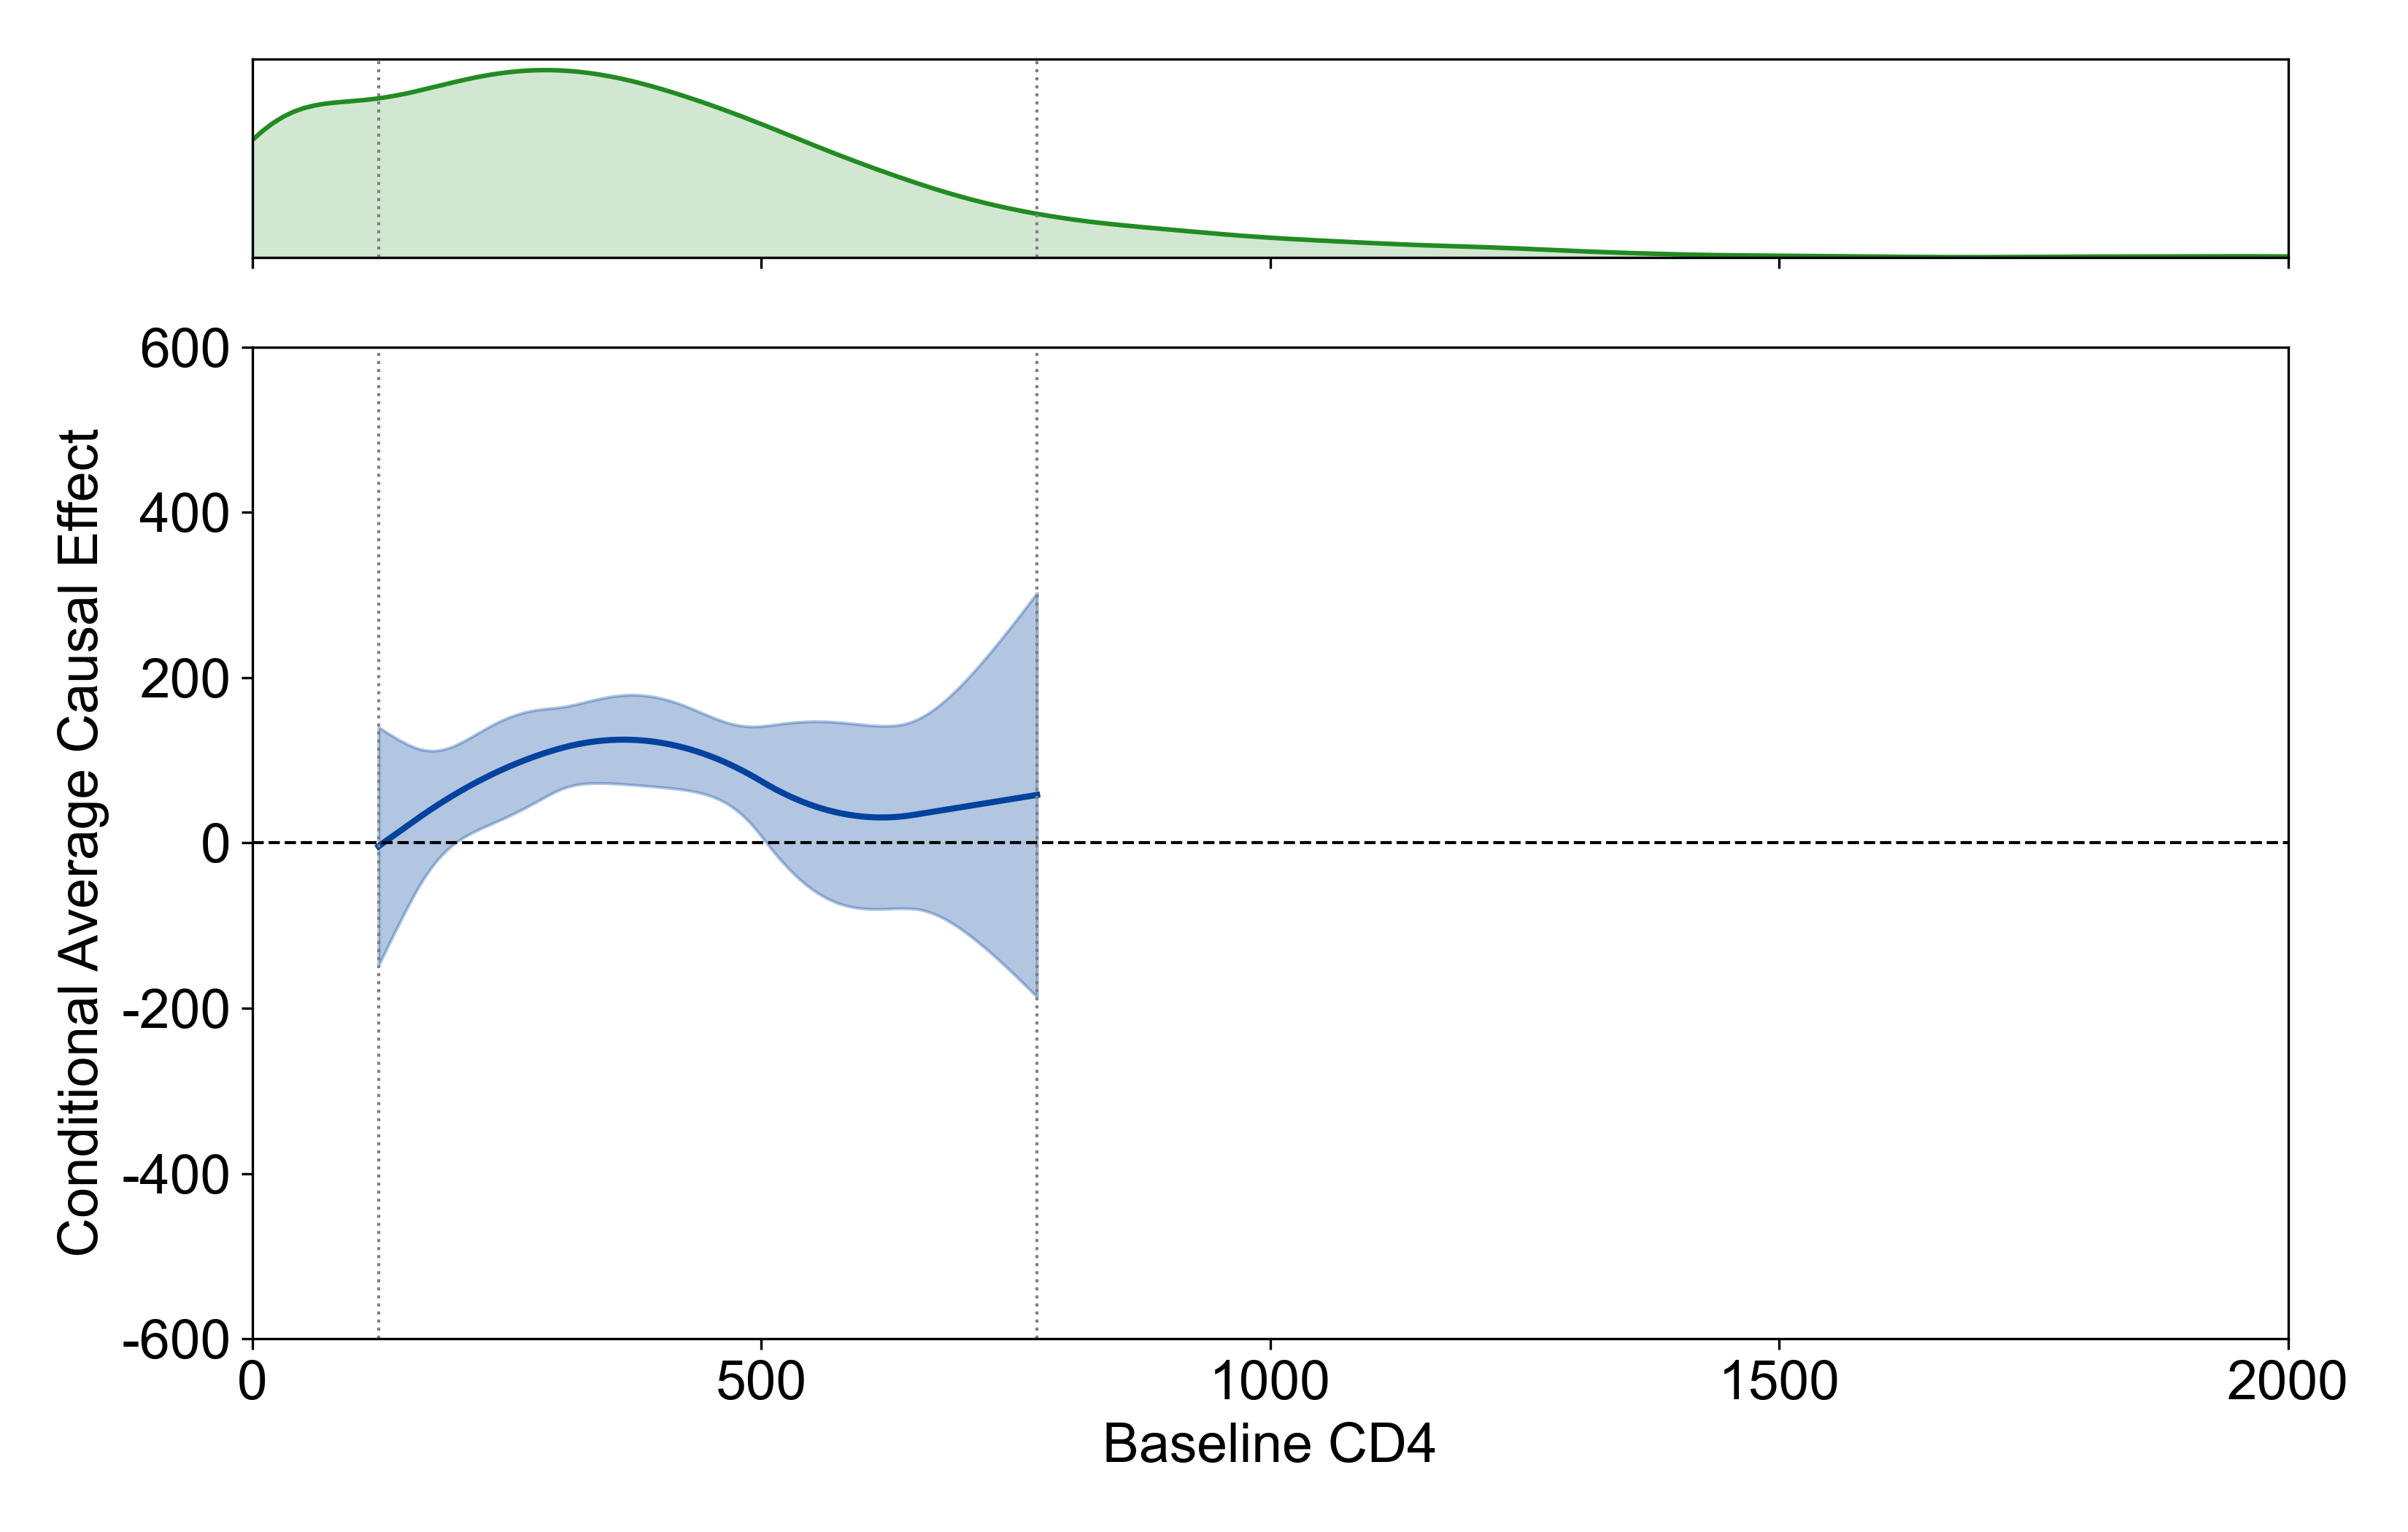
\includegraphics[width=0.85\linewidth]{images/cace_f0.png}
	\end{center}
\end{frame}

\begin{frame}{Challenge of Nonpositivity}
	\begin{center}
		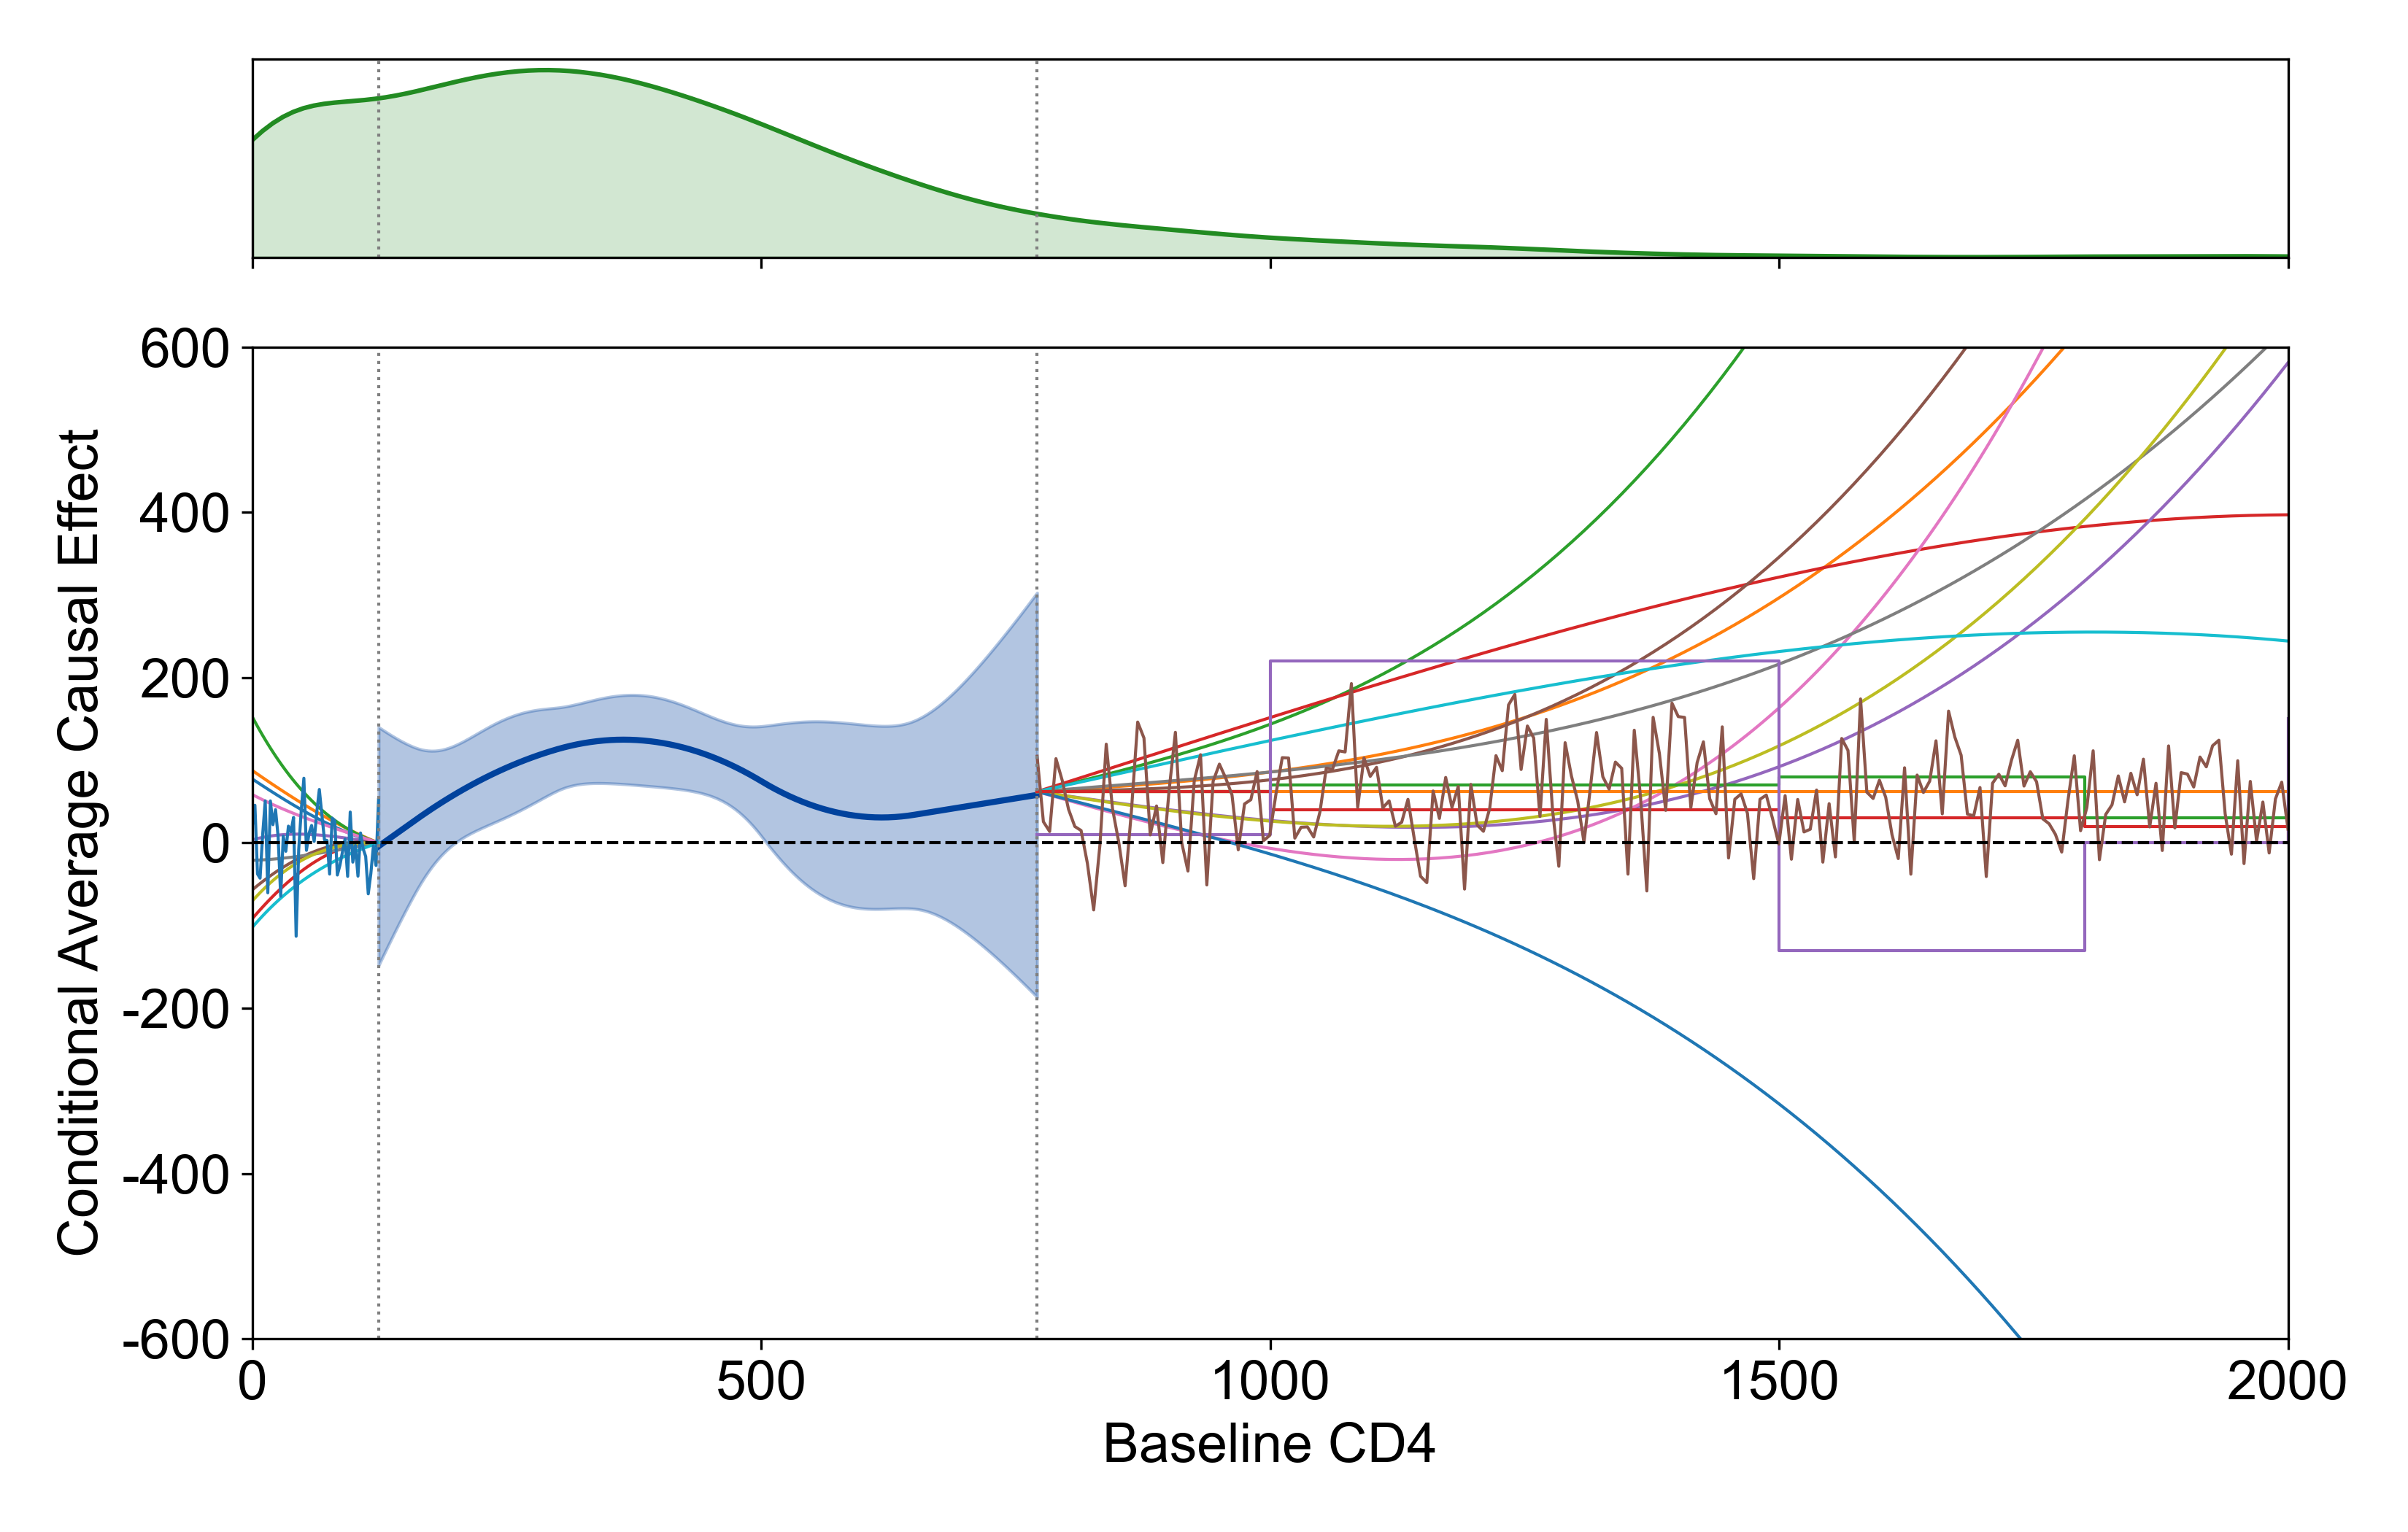
\includegraphics[width=0.85\linewidth]{images/cace_f1.png}	
	\end{center}
\end{frame}

\begin{frame}{Solution 1: Restrict Target Population}
	\begin{center}
		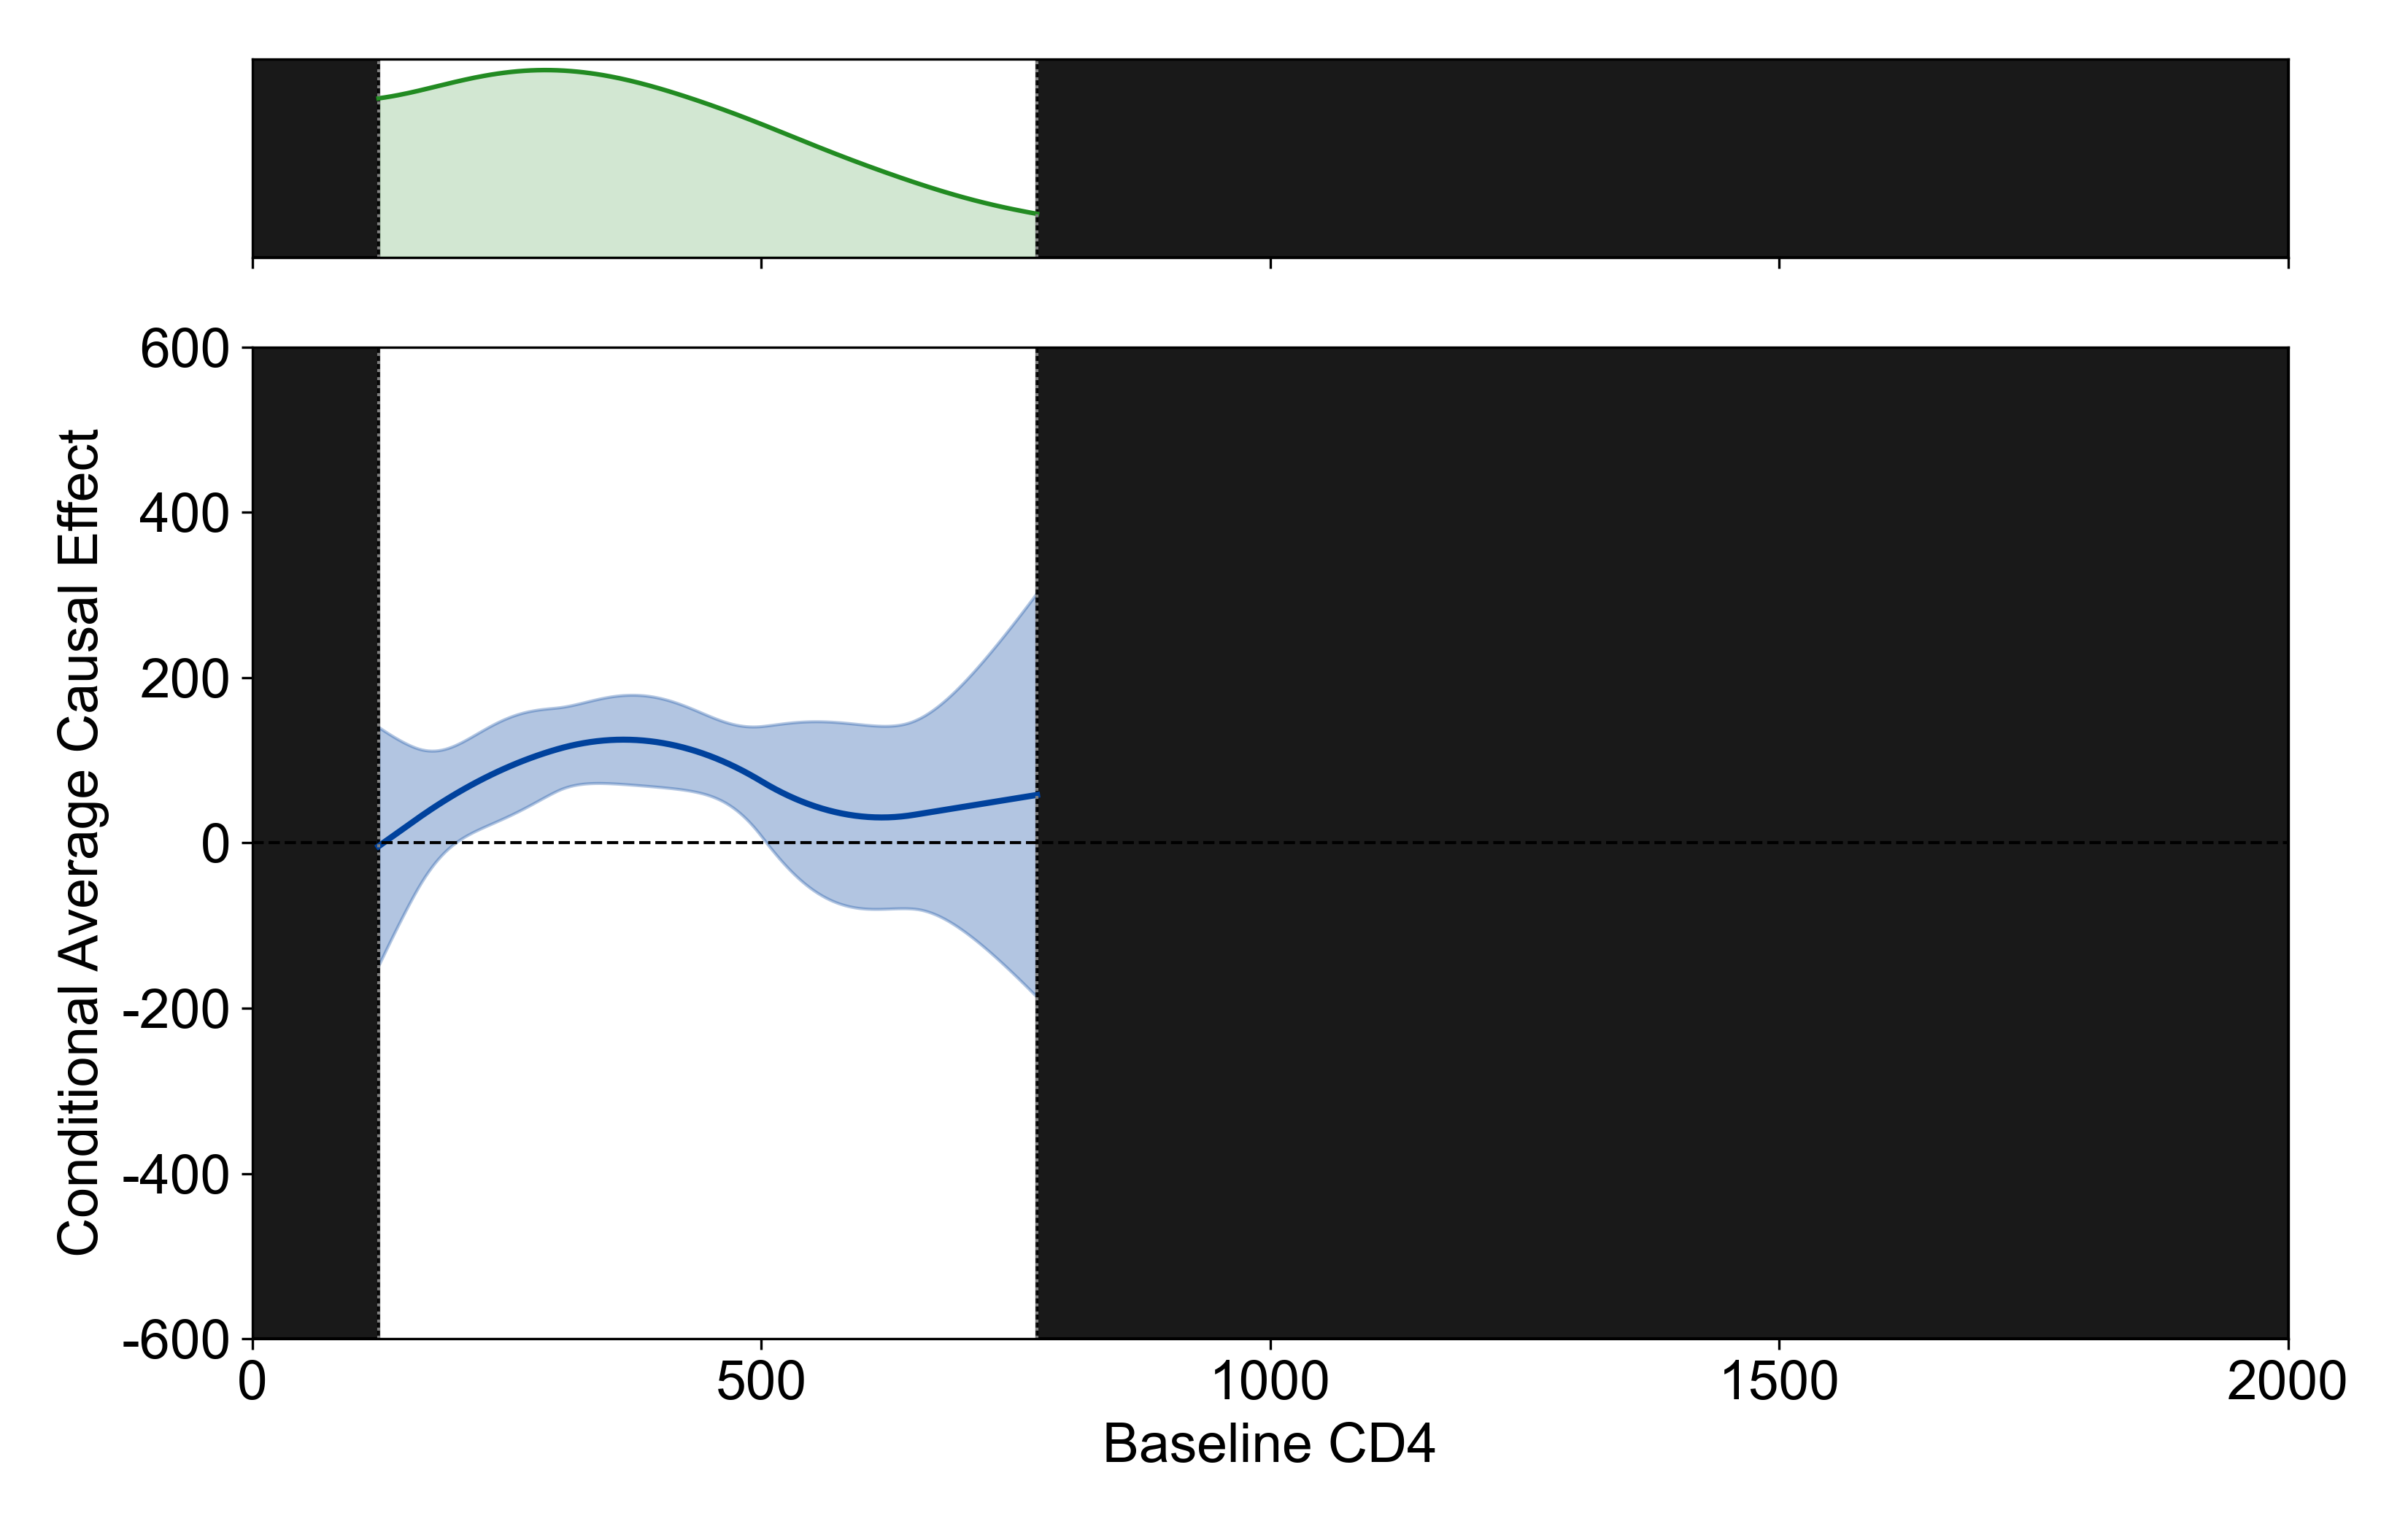
\includegraphics[width=0.85\linewidth]{images/cace_f2.png}	
	\end{center}
\end{frame}

\begin{frame}{Solution 2: Restrict Covariate Set}
	\begin{center}
		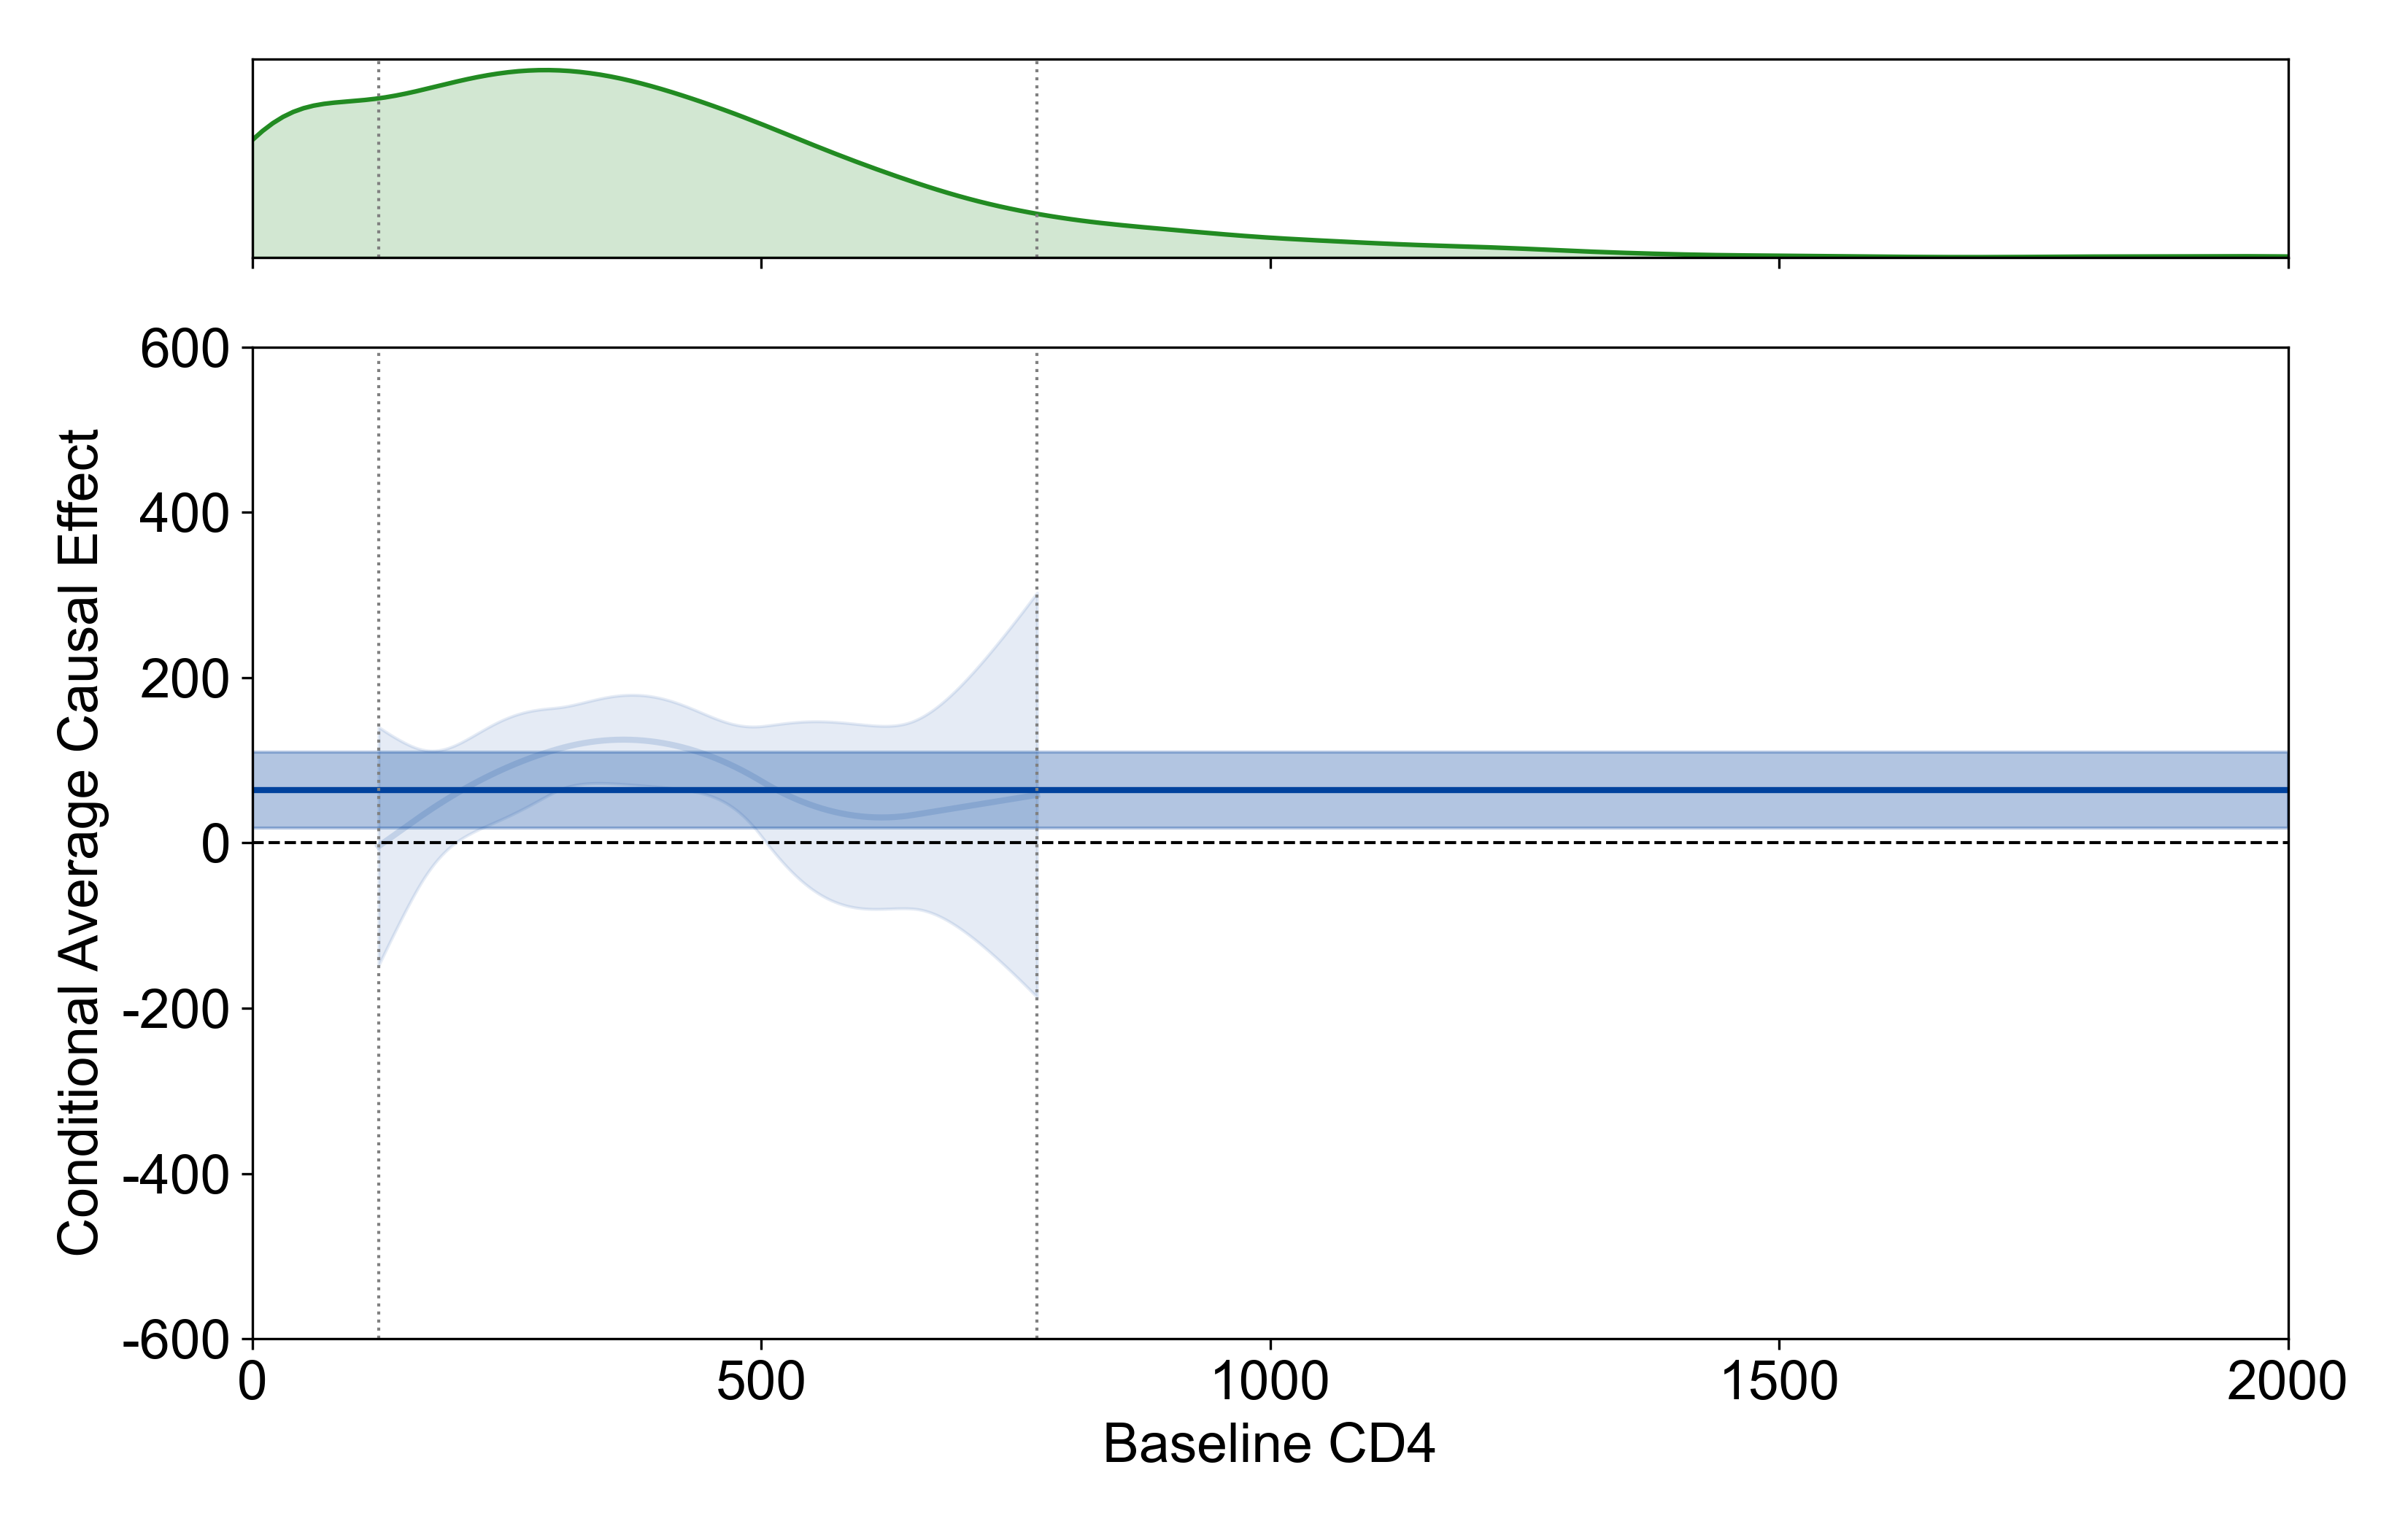
\includegraphics[width=0.85\linewidth]{images/cace_f3.png}	
	\end{center}
\end{frame}

\begin{frame}{Solution 3: Extrapolate}
	\begin{center}
		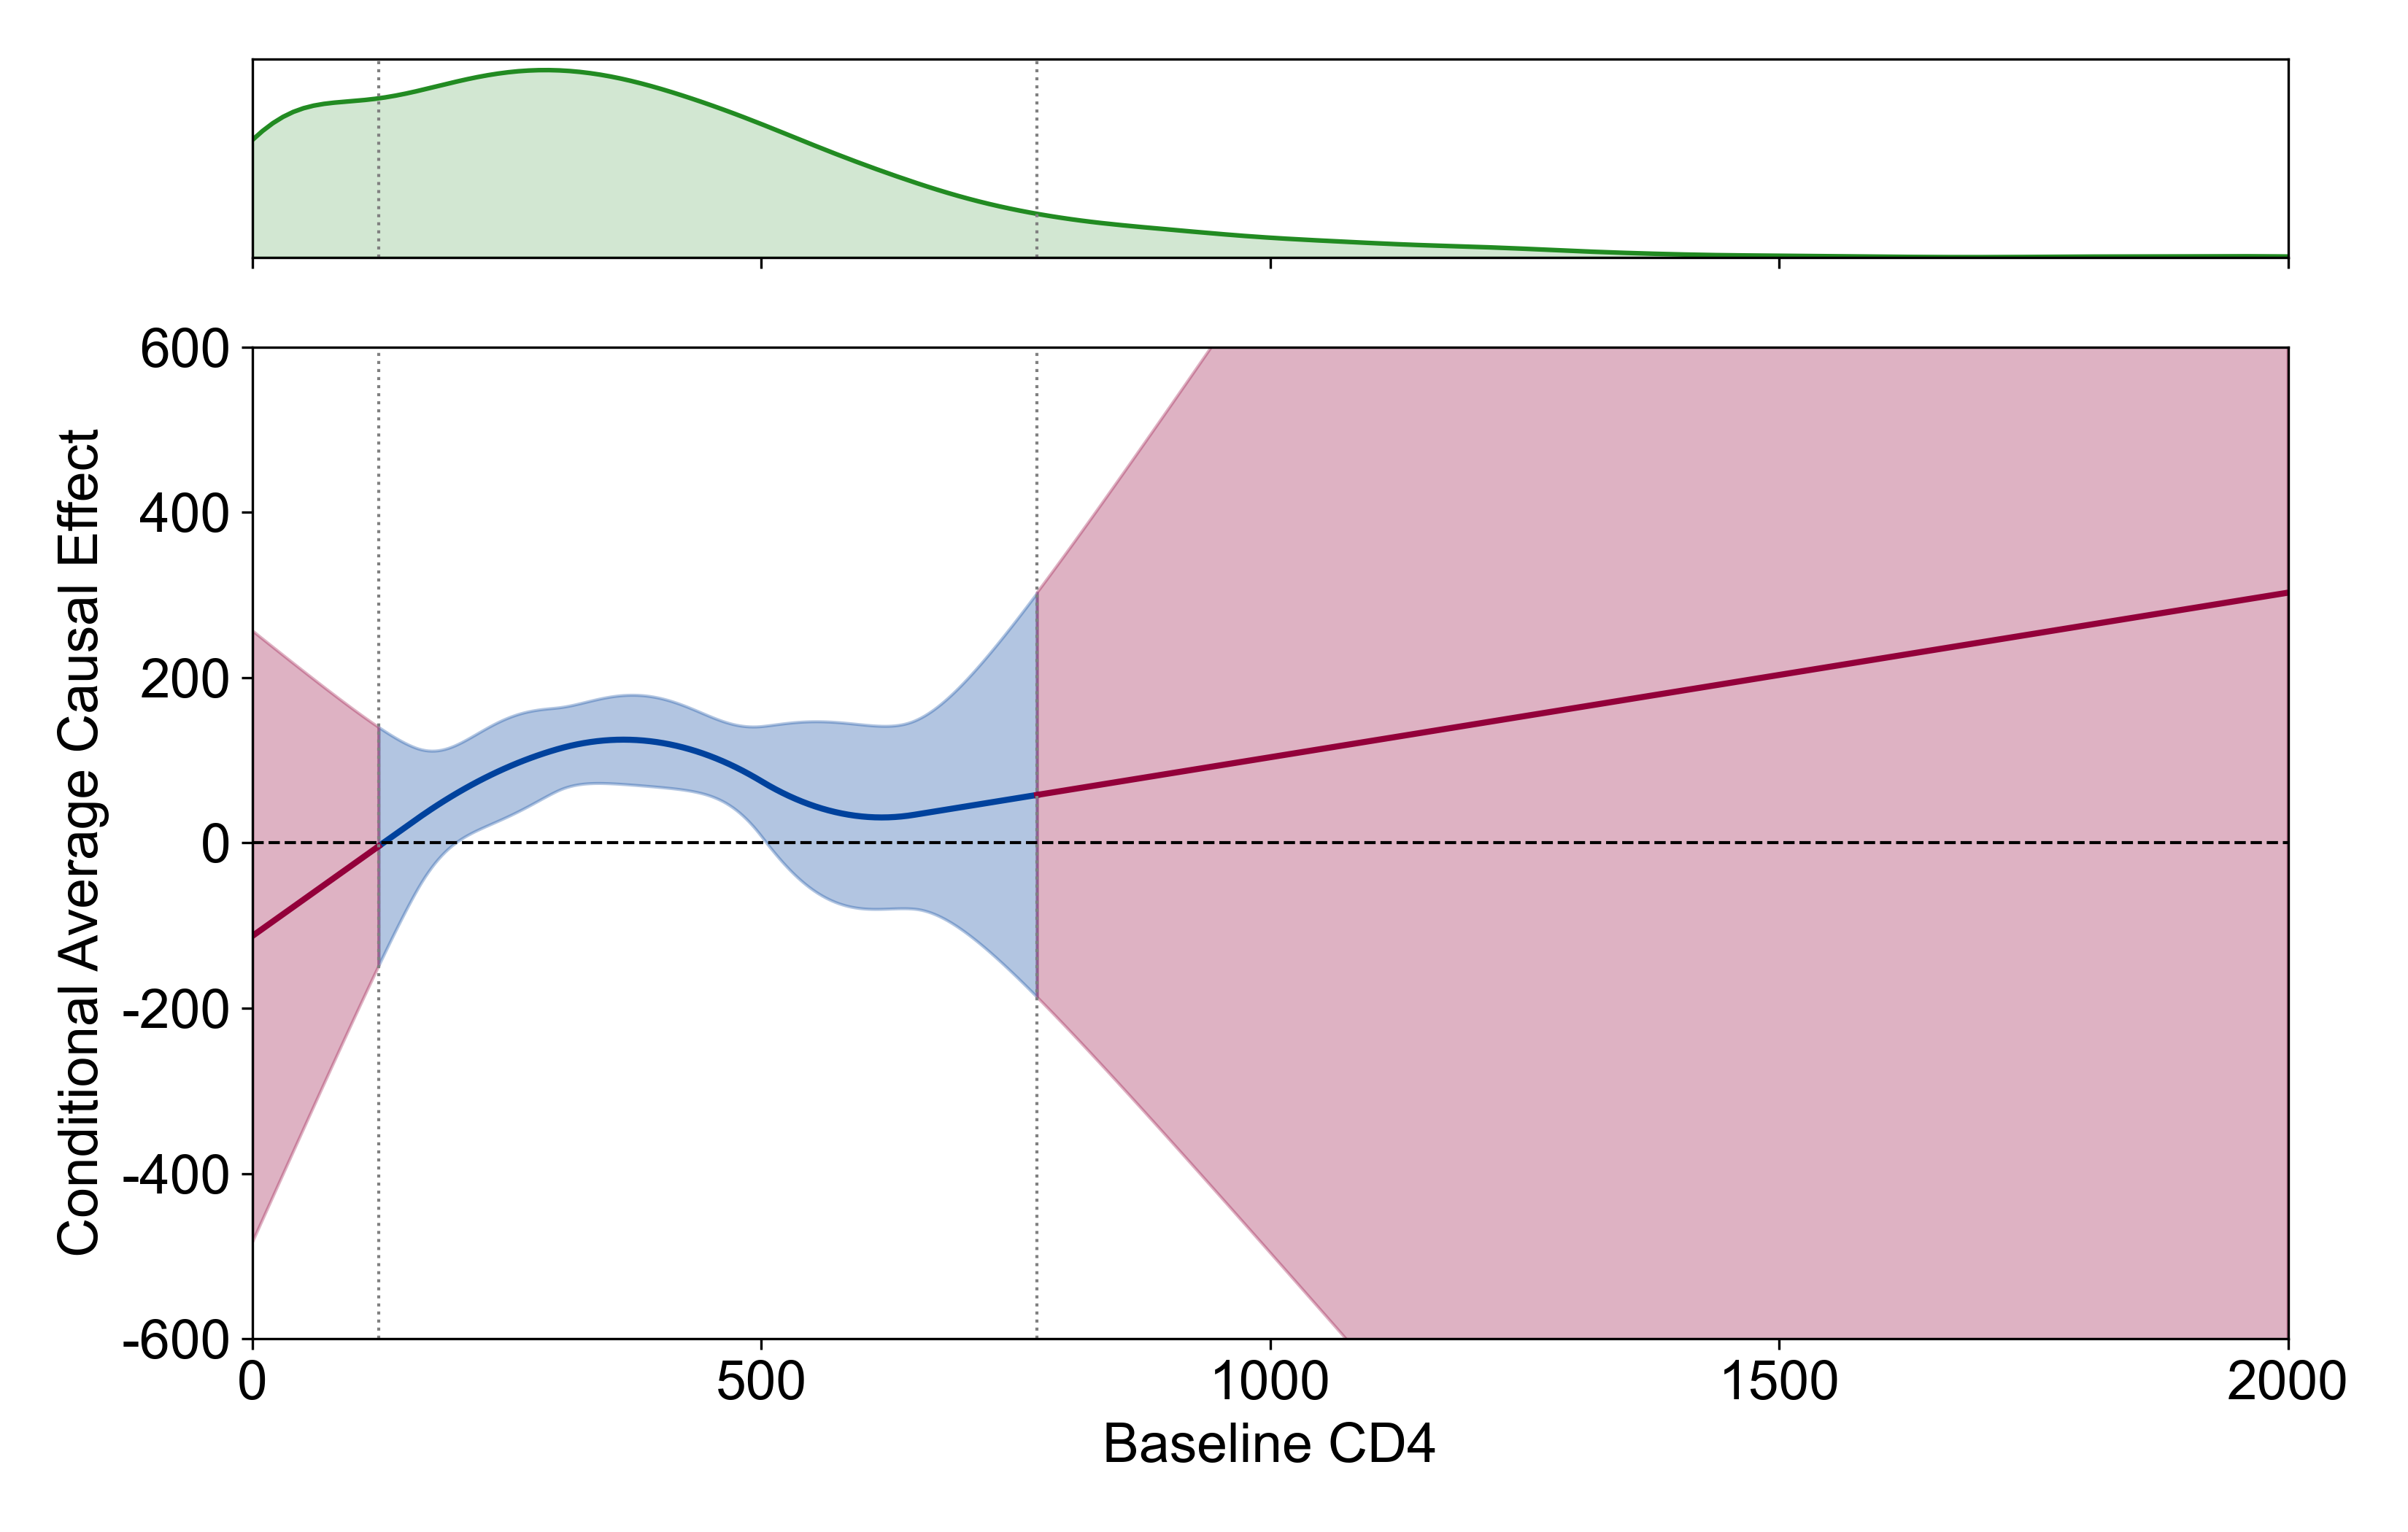
\includegraphics[width=0.85\linewidth]{images/cace_f4.png}	
	\end{center}
\end{frame}

\begin{frame}{Solution 4: Synthesis of Statistical and Mathematical Models}
	\begin{center}
		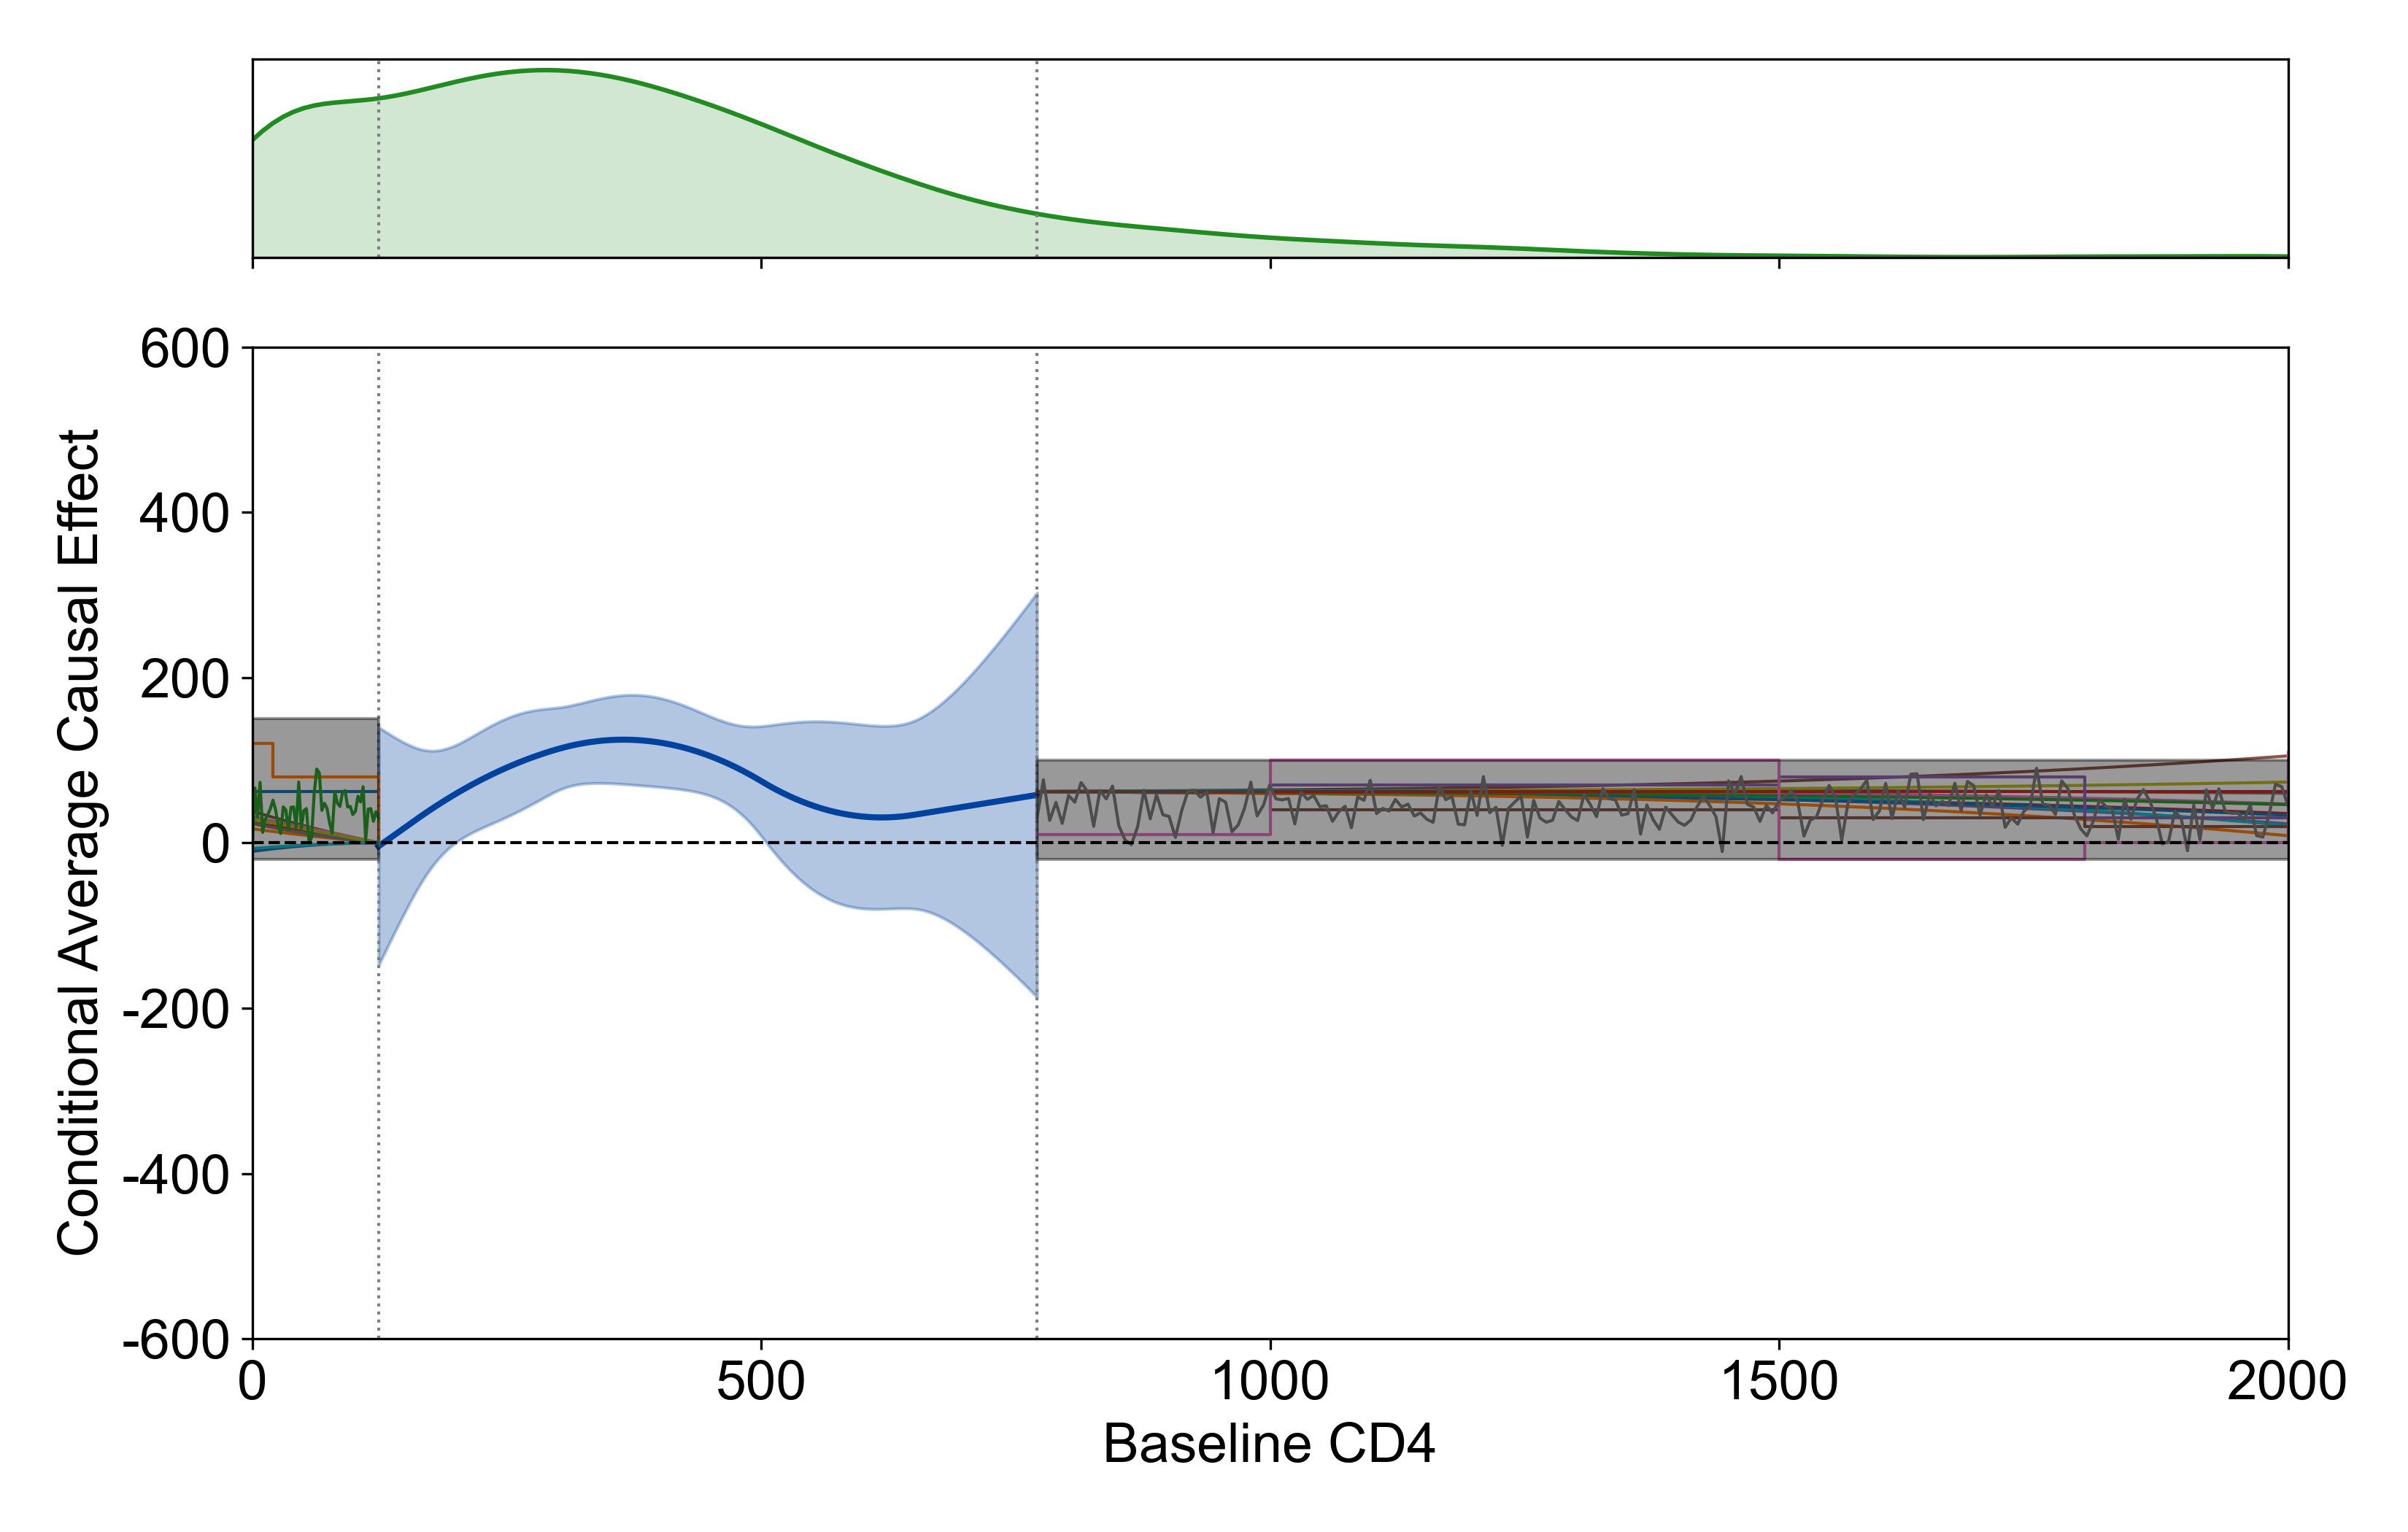
\includegraphics[width=0.85\linewidth]{images/cace_f6.png}	
	\end{center}
\end{frame}



\end{document}